\documentclass[12pt]{article}

\usepackage{booktabs}% http://ctan.org/pkg/booktabs
\usepackage[utf8]{inputenc}
\usepackage{changepage}
\usepackage{pgfplots}
\usepackage{amssymb}
\usepackage{xcolor}
\usepackage{hyperref}
\usepackage{listings}
\usepackage[T1]{fontenc}
\usepackage[utf8]{inputenc}
\usepackage{adjustbox}
\usepackage{amsmath}
\usepackage{mathtools}
\usepackage{biblatex}
\lstset{
  language=Python,
  numbers=left,
  numberstyle=\tiny,
  stepnumber=1,
  numbersep=5pt,
  tabsize=4,
  basicstyle=\ttfamily,
  columns=fullflexible,
  keepspaces,
}
\hypersetup{
    colorlinks,
    citecolor=black,
    filecolor=black,
    linkcolor=black,
    urlcolor=black
}

% Set page size and margins
% Replace `letterpaper' with `a4paper' for UK/EU standard size
\usepackage[letterpaper,top=2cm,bottom=2cm,left=3cm,right=3cm,marginparwidth=1.75cm]{geometry}

% Useful packages
\usepackage{amsmath}
\usepackage{mathtools}
\usepackage{graphicx}
\newenvironment{para}{\begin{adjustwidth}{13mm}{}}{\end{adjustwidth}}

\newcommand\tab[1][1cm]{\hspace*{#1}}

\newcommand{\tabitem}{\llap{\textbullet}}
\newcommand{\Hsquare}{%
\text{\fboxsep=-.2pt\fbox{\rule{0pt}{1ex}\rule{1ex}{0pt}}}%
}

\newtheorem{Definizione}{Definizione}[subsection]
\newtheorem{Lemma}{Lemma}[subsection]
\newtheorem{Teorema/Definizione}{Teorema/Definizione}[subsection]
\newtheorem{Corollario}{Corollario}[subsection]
\newtheorem{Teorema}{Teorema}[subsection]
\newtheorem{Proposizione}{Proposizione}[subsection]
\newtheorem{Notazione}{Notazione}[subsection]
\newtheorem{Commento}{Commento}[subsection]
\newtheorem{Dimostrazione}{Dimostrazione}[subsection]
\newtheorem{Osservazione}{Osservazione}[subsection]
\newtheorem{Nota}{Nota}[subsection]


\title{Analisi e Progettazione del Software}
\author{spitfire}
\date{A.A. 2023-2024}
\begin{document}
\begin{figure}
    \centering
    
\includegraphics[width=0.35\textwidth]{Images/Logo scienze bicocca.png}
\end{figure}

\vspace{10cm}
\date{A.A. 2023-2024}


\maketitle

\newpage

\tableofcontents
\newpage

\section{Introduzione}
Che cos'è il \textbf{software}? Esso è \textbf{un programma per computer} unito alla \textbf{documentazione ad esso associata},
la quale specifica e comprende \textbf{requisiti, modelli di progetto, manuale utente,...} \newline
I prodotti software possono essere:
\begin{itemize}
    \item \textbf{Generici}: sviluppati per un ampio insieme di clienti (elaboratori di testo, database,...)
    \item \textbf{Personalizzati} (custom): sviluppati per un singolo cliente in base alla sue esigenze specifiche
\end{itemize}
Un nuovo prodotto software può essere \textbf{creato da zero, personalizzando software già esistenti o riusando parti o software già esistente}.
Le caratteristiche essenziali di un buon software sono:
\begin{center}
    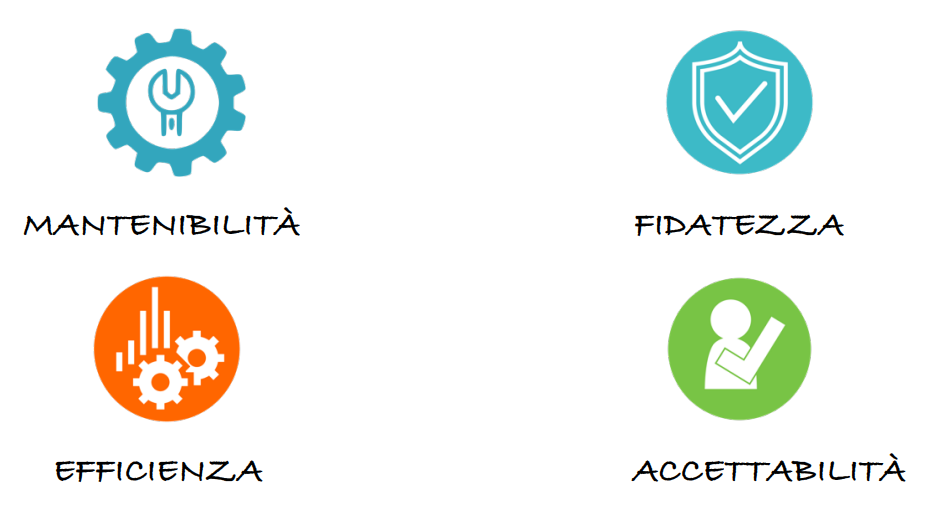
\includegraphics[width = 0.80\textwidth]{Images/1.png}
\end{center}
\subsection{Introduzione all'ingegneria del software}
Che cos'è \textbf{l'ingegneria del software}? \textbf{L'ingegneria del software} è una disciplina ingegneristica che si occupa
di tutti gli aspetti della produzione del software di buona qualità, dalle \textbf{prime fasi della specifica del sistema fino alla manutenzione del sistema}
dopo la messa in uso. Vediamo cosa si intende per \textbf{disciplina ingegneristica} e "\textbf{Tutti gli aspetti della produzione del software}":
\begin{itemize}
    \item \textbf{Disciplina ingegneristica}: Utilizzare metodi e teorie \textbf{appropriati} per risolvere i problemi tenendo conto dei vincoli \textbf{organizzativi e finanziari}
    \item \textbf{Tutti gli aspetti della produzione del software}: Non solo il \textbf{processo tecnico di sviluppo}. Anche la \textbf{gestione del progetto} e lo sviluppo di \textbf{strumenti}
    ,metodi ecc... per supportare la produzione del software
\end{itemize}
\newpage
\noindent
La disciplina dell'ingegneria del software si occupa di:
\begin{center}
    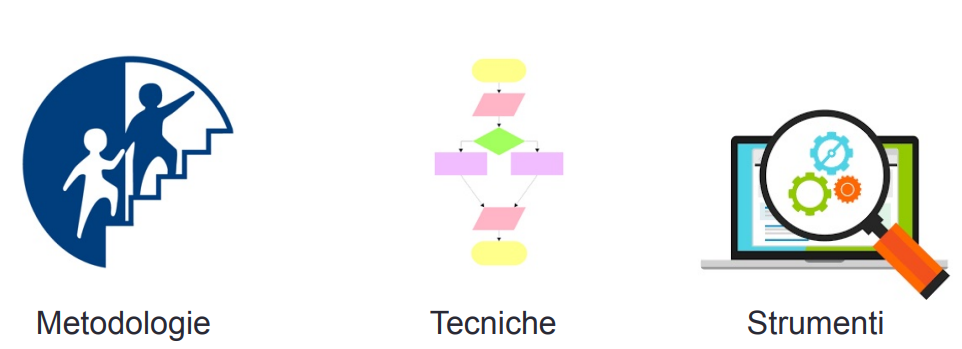
\includegraphics[width = 0.80\textwidth]{Images/2.png}
\end{center}
\subsection{La crisi del software}
Il termine \textbf{crisi del software} (o software crisis) è usato nell'ambito dell'ingegneria del software per descrivere l'impatto della \textbf{rapida crescita} della potenza degli elaboratori
e la \textbf{complessità} dei problemi che dovevano esseri affrontati. Le parole chiavi della software crisis erano \textbf{complessità, attese e cambiamento}. Il concetto di software crisis emerse negli
anni '60.
\begin{center}
    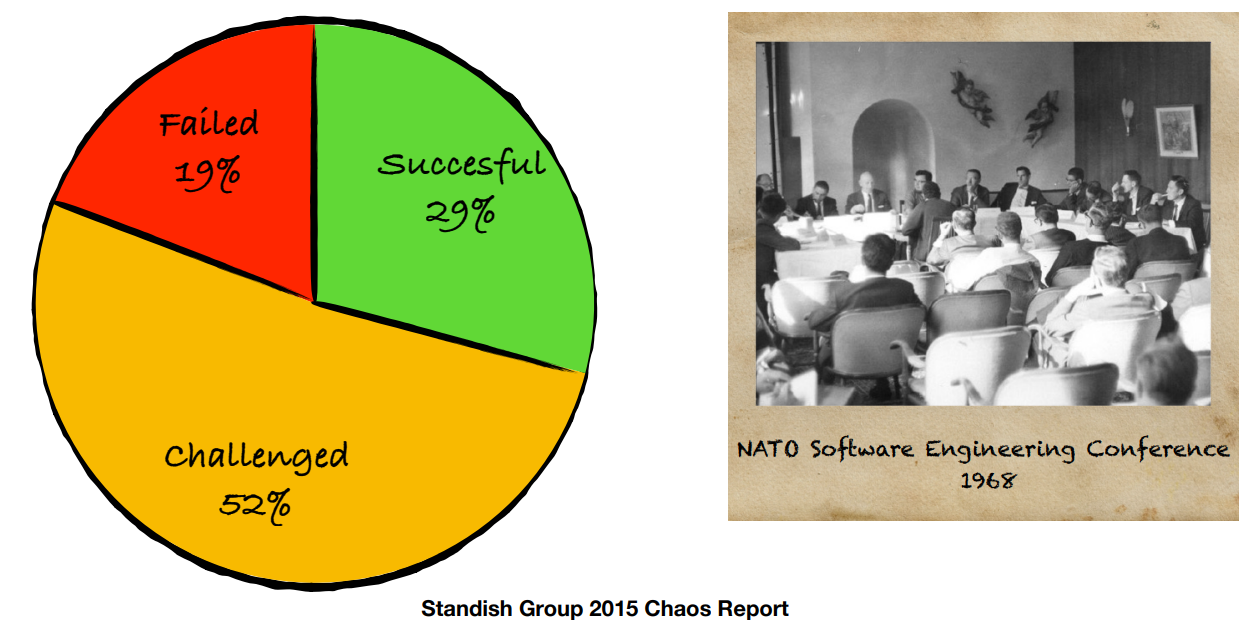
\includegraphics[width = 0.80\textwidth]{Images/3.png}
\end{center}
\begin{center}
    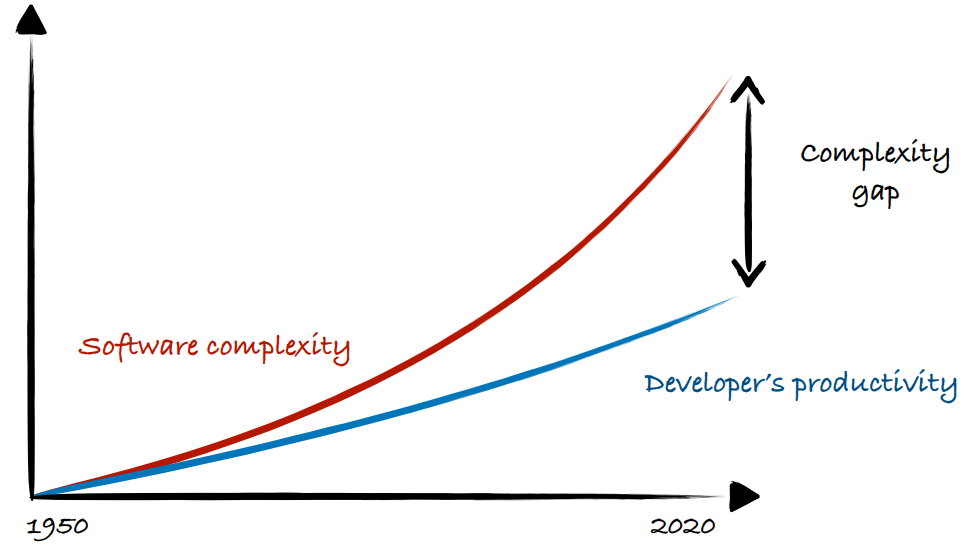
\includegraphics[width = 0.80\textwidth]{Images/4.png}
\end{center}
Le cause della crisi del software erano legate alla \textbf{complessità dei processi software} e alla \textbf{relativa immaturità dell'ingegneria del software}
Per superare la crisi infatti si dovettero introdurre:
\begin{itemize}
    \item \textbf{Management}
    \item \textbf{Organizzazione}, attraverso \textbf{analisi e progettazione}
    \item \textbf{Teorie e tecniche} come la \textbf{programmazione strutturata e ad oggetti}
    \item \textbf{Strumenti}, come gli IDE
    \item \textbf{Metodologie}, tra cui il \textbf{modello a cascata e il modello agile}
\end{itemize}
\subsection{Analisi e progettazione}
Che cosa sono \textbf{analisi e progettazione}? \newline
\textbf{L'analisi} enfatizza un'\textbf{investigazione del problema e dei requisiti} invece che una soluzione: per esempio, se si vuole realizzare un nuovo sistema di trading online,
bisognerà capire \textbf{come questo sistema verrà utilizzato} e \textbf{quali sono le sue funzioni}. "Analisi" è un termine ampio con più accezioni, tra cui:
\begin{itemize}
    \item \textbf{Analisi dei requisiti}, cioè un'investigazione dei requisiti del sistema
    \item \textbf{Analisi orientata agli oggetti}, cioè un'investigazione degli oggetti di dominio
\end{itemize} 
La \textbf{progettazione} enfatizza una soluzione \textbf{concettuale} (software e hardware) che \textbf{soddisfa i requisiti}, anziché la relativa implementazione. Per esempio, la descrizione di uno schema di base di dati
e di oggetti software. Nella progettazione vengono spesso \textbf{esclusi dettagli di basso livello o "ovvi"} (o almeno "ovvi" per coloro a cui è destinato il software). \newline
Infine i progetti possono essere \textbf{implementati} e la loro implementazione (ovvero il codice) esprime il progetto realizzato vero e completo.
Come nel caso dell'analisi, anche "progettazione" è un termine con più accezioni, tra cui:
\begin{itemize}
    \item \textbf{Progettazione orientata agli oggetti}
    \item \textbf{Progettazione di basi di dati}
\end{itemize}
L'analisi e la progettazione possono essere riassunti con la seguente frase:
\begin{center}
    \textbf{Fare la cosa giusta}(analisi) \textbf{e fare la cosa bene}(progettazione)
\end{center}
\subsubsection{Analisi e progettazione orientata agli oggetti}
Durante \textbf{l'analisi orientata agli oggetti} c'è un enfasi sull'\textbf{identificazione} e la \textbf{descrizione degli oggetti}, o dei \textbf{concetti}, nel \textbf{dominio del problema}.
Per esempio, nel caso di un sistema informatico per voli aerei, alcuni dei concetti possono essere \textit{Aereo, Volo} e \textit{Pilota}. \newline
Durante \textbf{la progettazione orientata agli oggetti} (o più semplicemente \textbf{progettazione a oggetti}) l'enfasi è sulla \textbf{definizione di oggetti software} e sul \textbf{modo in cui questi collaborano
per soddisfare i requisiti}. Per esempio un oggetto software \textit{Aereo} può avere un attributo \textit{codiceDiRegistrazione} e un metodo \textit{getVoliEffettuati}. \newline
\begin{center}
    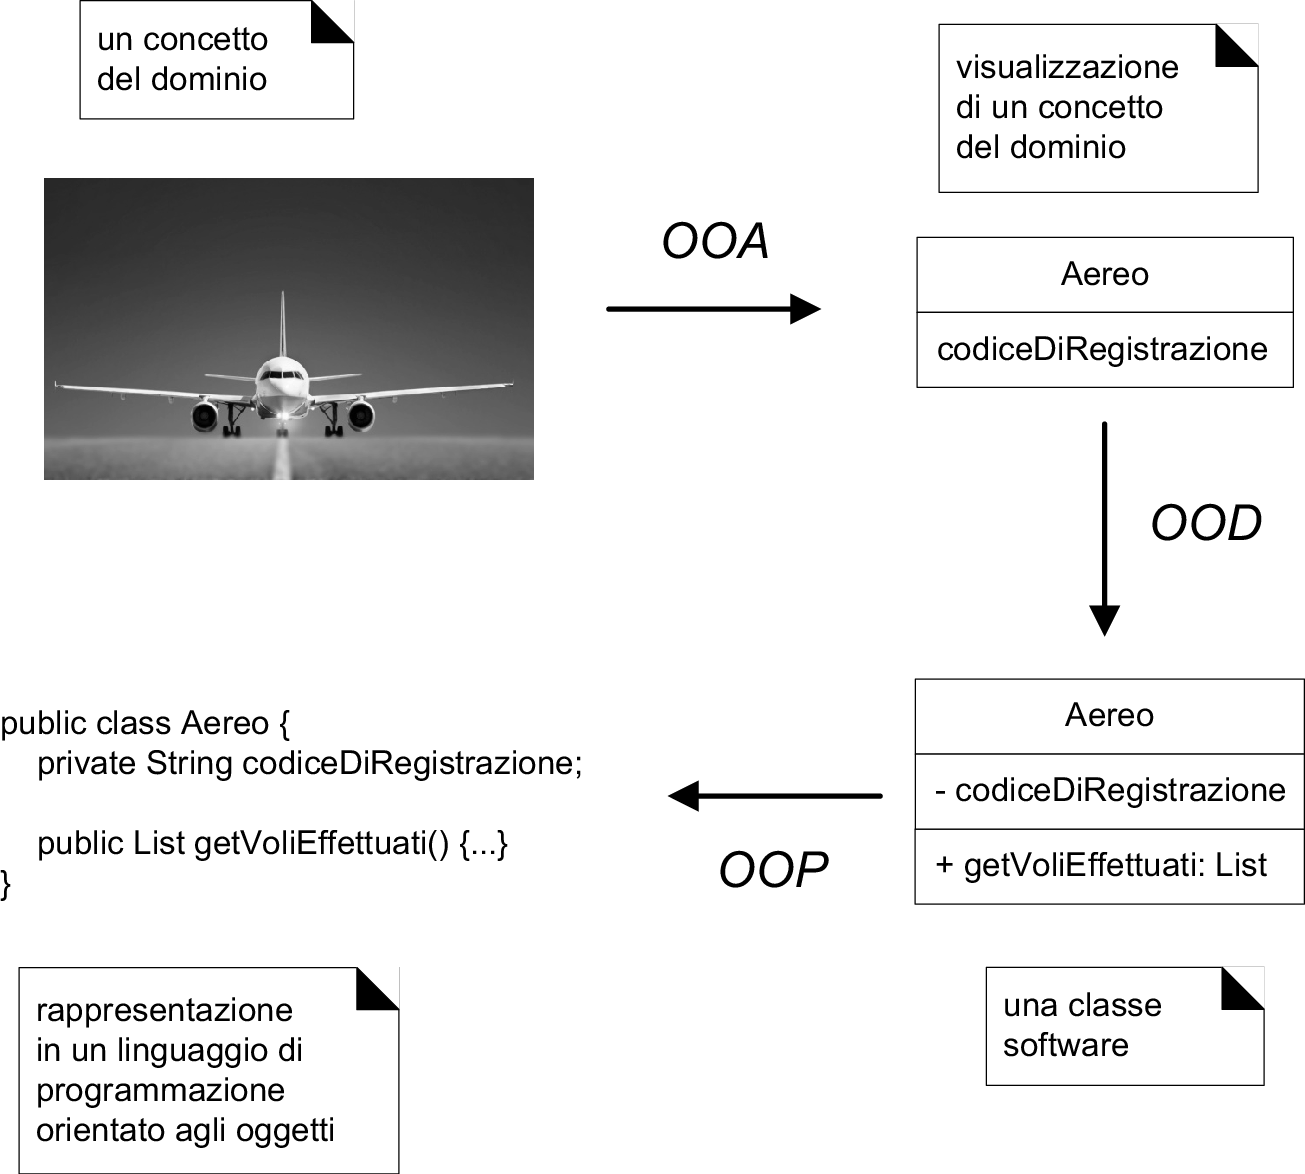
\includegraphics[width = 0.70\textwidth]{Images/5.png}
\end{center}
Infine durante \textbf{l'implementazione} o la \textbf{programmazione orientata agli oggetti}, gli oggetti progettati vengono implementati, per esempio implementando la classe \textit{Aereo} in un linguaggio ad oggetti.
Dunque, analisi e progettazione \textbf{hanno obbiettivi diversi che vengono perseguiti in maniera diversa}. Tuttavia, come mostrato dall'esempio sopra, esse sono \textbf{attività fortemente sinergiche} che sono \textbf{correlate fra loro}
e con le \textbf{altre attività dello sviluppo del software}.
\subsection{Introduzione ai diagrammi e ai passi fondamentali dello sviluppo software}
Vediamo una breve introduzione dei \textbf{vai diagrammi e dei passi fondamentali} legati allo sviluppo software.
\begin{center}
    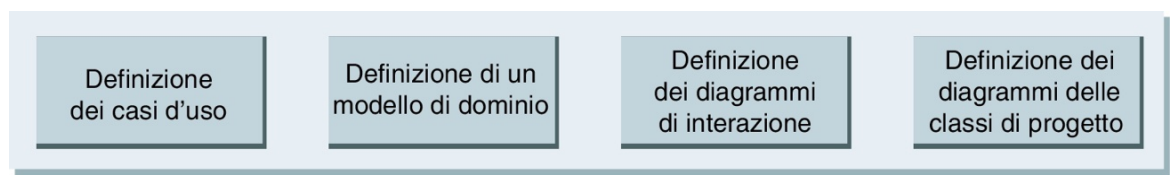
\includegraphics[width = 0.80\textwidth]{Images/6.png}
\end{center}
\subsubsection{Definizione dei casi d'uso}

\textbf{L'analisi dei requisiti} può comprendere \textbf{storie o scenari} relativi al modo in cui l'applicazione può essere utilizzata dagli utenti;
queste storie possono essere scritte come \textbf{casi d'uso}. I casi d'uso \textbf{non sono un elaborato ad oggetti} ma semplicemente delle storie scritte. Sono tuttavia
uno strumento \textbf{diffuso nell'analisi dei requisiti}. Facciamo un'esempio: \newline
\textbf{Gioca una partita a Dadi}: Il giocatore chiede di lanciare i dadi. Il Sistema presenta il risultato: se il valore totale delle facce dei dadi è sette, il giocatore ha vinto; altrimenti ha perso.
\subsubsection{Definizione di un modello di dominio}
L'analisi orientata agli oggetti è interessata alla \textbf{creazione di una descrizione del dominio da un punto di vista ad oggetti}. Vengono identificati i \textbf{concetti, gli attributi e le associazioni considerati significativi}.
Il risultato può essere espresso come un \textbf{modello di dominio} che mostra i concetti o gli oggetti \textbf{significativi} del dominio. Esso è rappresentato nel seguente modo:
\begin{center}
    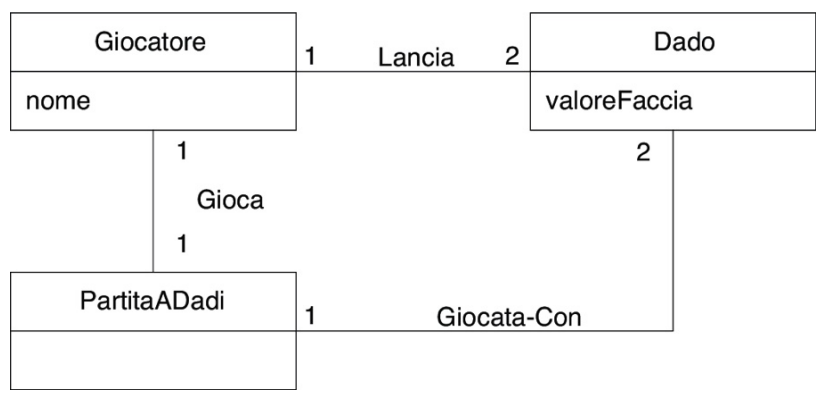
\includegraphics[width = 0.65\textwidth]{Images/7.png}
\end{center}
\subsubsection{Definizione dei diagrammi di interazione}
La \textbf{progettazione ad oggetti} è interessata alla \textbf{definizione di oggetti software, delle loro responsabilità e collaborazioni}. Una notazione comune per illustrare queste collaborazione è un
\textbf{diagramma di sequenza} (un tipo di diagramma UML). Esso mostra lo scambio di messaggi \textbf{tra oggetti software}, dunque l'invocazione di \textbf{metodi}. Esso è rappresentato nel seguente modo:
\begin{center}
    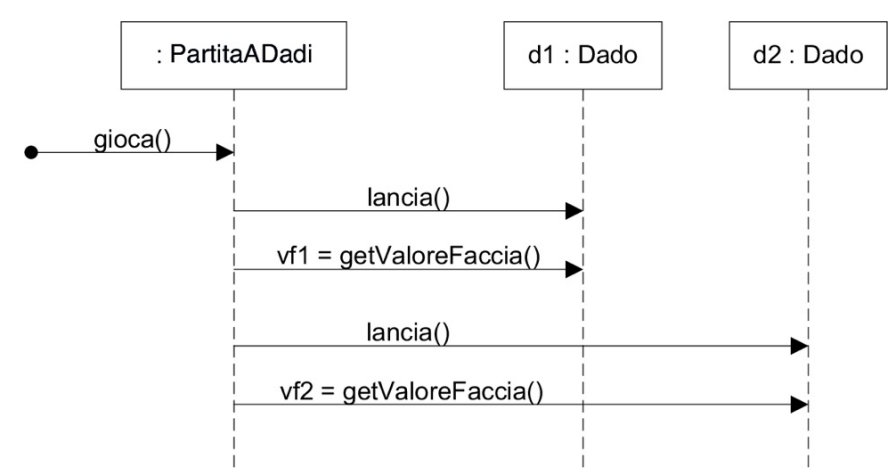
\includegraphics[width = 0.65\textwidth]{Images/8.png}
\end{center}
È interessante notare come \textbf{la progettazione degli oggetti software e dei programmi si può ispirare a un dominio del mondo reale}, tuttavia essa non è \textbf{nè un modello diretto nè una simulazione di questo dominio}. Quindi, per esempio,
seppur nel mondo reale è il giocatore a lanciare il dado, nel progetto software è l'oggetto \textit{PartitaADadi} che "lancia" i dadi.
\subsubsection{Definizione dei diagrammi di classe di progetto}
Accanto a una visione dinamica delle \textbf{collaborazioni tra oggetti}, mostrata dai diagrammi di interazione, è utile mostrare una \textbf{vista statica} delle definizioni di classi mediante un \textbf{diagramma delle classi di progetto}, che mostra le classi software 
con i loro attributi e metodi. Il diagramma delle classi di progetto è rappresentato nella seguente maniera:
\begin{center}
    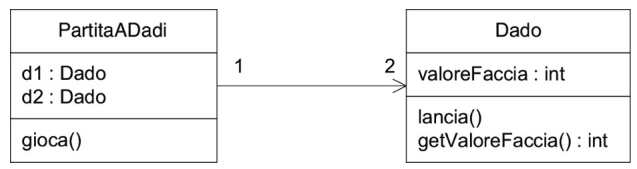
\includegraphics[width = 0.65\textwidth]{Images/9.png}
\end{center}
Diversamente dal modello di dominio, che illustra \textbf{classi del mondo reale}, questo diagramma mostra \textbf{classi software}.
Si noti che, benché questo diagramma delle classi di progetto \textbf{non sia uguale al modello di dominio}, i nomi e il contenuto delle classi sono \textbf{simili}. In tal modo i \textbf{progetti e i linguaggi Object Oriented} (OO) sono in grado di \textbf{favorire un salto rappresentazionale basso}
tra i componenti software e il nostro modello mentale di un dominio, \textbf{migliorando la comprensione}.
\subsection{UML}
\textbf{Unified Modelling Language}, abbreviato \textbf{UML}, è un \textbf{linguaggio visuale} per la \textbf{specifica, la costruzione e la documentazione degli elaborati} di un sistema software.
UML rappresenta una \textbf{collezione di best practices di ingegneria}, dimostratesi vincenti nella modellazione di sistemi vasti e complessi; inoltre esso \textbf{favorisce la divulgazione delle informazioni nella comunità dell'ingegneria del software} in quanto è \textit{standard de facto}.
Bisogna però tenere a mente che \textbf{UML non è una metodologia ma un linguaggio!} \newline
Il termine \textit{visuale} della definizione è un punto fondamentale. UML è uno standard de facto per la \textbf{notazione di diagrammi per disegnare o rappresentare figure} (con del testo) \textbf{relative al software}, e in particolare, al software OO.
A un livello più profondo, di particolare interesse per i produttori di strumenti per \textbf{MDA} (Model Driven Architecture) alla base della notazione UML c'è il \textbf{meta-modello di UML} che descrive la \textbf{semantica} degli elementi di modellazione, tuttavia non è necessario che lo sviluppatore lo conosca. 
Presentiamo ora una breve storia di UML:
\begin{center}
    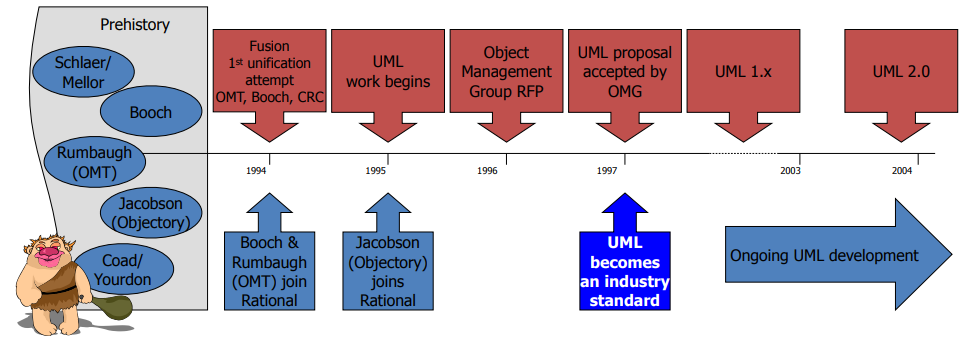
\includegraphics[width = 1.05\textwidth]{Images/10.PNG}
\end{center}
Il più significativo aggiornamento di UML è avvenuto nel \textbf{2003}:
\begin{itemize}
    \item Maggiore \textbf{consistenza}
    \item Semantica definita in maniera \textbf{più chiara e dettagliata}
    \item \textbf{Nuovi diagrammi}
    \item Compatibilità con le precedenti versioni (1.x)
\end{itemize}
Altra parola importante è \textit{unified}: UML vuole essere un \textbf{linguaggio unificante} sotto diversi aspetti:
\begin{itemize}
    \item \textbf{Storico} (OMT, Booch, CRC, Objectory)
    \item \textbf{Ciclo di sviluppo} (sintassi visuali per tutte le fasi)
    \item \textbf{Domini applicativi} (dai sistemi embedded ai sistemi gestionali)
    \item \textbf{Linguaggi e piattaforme di sviluppo} (.Net, Java, C\#,...)
    \item \textbf{Processi di sviluppo} (UP, BPM, ...)
\end{itemize}
\subsubsection{UML e gli oggetti}
UML modella i sistemi come \textbf{una serie di oggetti che collaborano fra loro}. Si hanno quindi due strutture:
\begin{itemize}
    \item \textbf{Struttura statica}:
    \begin{itemize}
        \item \textbf{Quali} tipi di oggetti sono necessari
        \item \textbf{Come} sono correlati
    \end{itemize}
    \item \textbf{Struttura dinamica}:
    \begin{itemize}
        \item \textbf{Ciclo di vita} di questi oggetti
        \item \textbf{Come collaborano} per fornire le funzionalità richieste
    \end{itemize}
\end{itemize}
\subsubsection{Tre modi di applicare UML}
\textbf{Fowler} [Fowler03] descrive tre modi per applicare UML:
\begin{itemize}
    \item \textbf{UML come abbozzo}: Diagrammi \textbf{informali e incompleti} (spesso abbozzati a mano su una lavagna bianca), che vengono creati per 
    \textbf{esplorare parti difficili dello spazio del problema o della soluzione}, sfruttando l'espressività dei linguaggi visuali.
    \item \textbf{UML come progetto}: Diagrammi di progetto abbastanza dettagliati che vengono utilizzati per:
    \begin{enumerate}
        \item \textbf{Il reverse engineering}, ovvero per visualizzare e comprendere meglio \textbf{del codice già esistente} mediante dei diagrammi UML. In questo caso, uno strumento UML legge il codice
        sorgente o binario per \textbf{generare} (di solito) \textbf{dei diagrammi UML dei package, delle classi e di sequenza}. Questi "progetti" possono aiutare il lettore a capire i principali elementi, le strutture e le collaborazioni
        \item \textbf{Il forward engineering}, ovvero per la \textbf{generazione di codice}. In questo caso, alcuni diagrammi dettagliati possono fornire una \textbf{guida alla generazione di codice} da fare manualmente o automaticamente con un strumento.
        Solitamente, i diagrammi sono utilizzati per \textbf{specificare una parte di codice}, mentre il resto del codice viene scritto da uno sviluppatore durante la codifica, magari applicando UML come abbozzo.
    \end{enumerate}
    \item \textbf{UML come linguaggio di programmazione}: La specifica \textbf{completamente eseguibile} di un sistema software con UML.
    Il codice viene generato \textbf{automaticamente} e non viene normalmente normalmente né visto né modificato dagli sviluppatori; quindi UML viene usato come vero e proprio \textbf{linguaggio di programmazione}.
    Questo utilizzo di UML richiede un modo \textbf{pratico} per rappresentare sotto forma di di diagrammi \textbf{tutto il comportamento o la logica} (probabilmente tramite diagrammi di interazione e di stato).
    Si tratta di un approccio \textbf{ancora in corso di sviluppo} sia in termini di teoria sia in termini di usabilità e robustezza degli strumenti.
\end{itemize}
La \textbf{modellazione agile} enfatizza l'uso di UML come \textbf{abbozzo}; si tratta di un metodo comune per applicare UML, spesso con un elevato ritorno in termini di \textbf{investimento di tempo} (che è normalmente breve).
\subsubsection{Due punti di vista per applicare UML}
UML descrive dei tipi \textbf{grezzi} di diagrammi, come i diagrammi delle classi e i diagrammi di sequenza; tuttavia UML \textbf{non impone un particolare punto di vista di modellazione per l'uso di questi diagrammi}; 
quindi la stessa notazione può essere usata secondo \textbf{due punti di vista} (o prospettive) e \textbf{tipi di modelli}:
\begin{itemize}
    \item \textbf{Punto di vista concettuale}: I diagrammi sono scritti e interpretati \textbf{come descrizioni di oggetti del mondo reale} o nel dominio di interesse
    \item \textbf{Punto di vista software}: I diagrammi, che utilizzano \textbf{la stessa notazione del punto di vista concettuale}, descrivono astrazioni o componenti software. In particolare, i diagrammi possono descrivere:
    \begin{enumerate}
        \item \textbf{Implementazioni software} con riferimento a una particolare tecnologia
        \item \textbf{Specifiche e interfacce} di componenti software, ma \textbf{indipendentemente} da ogni possible implementazione
    \end{enumerate}
\end{itemize}
\begin{center}
    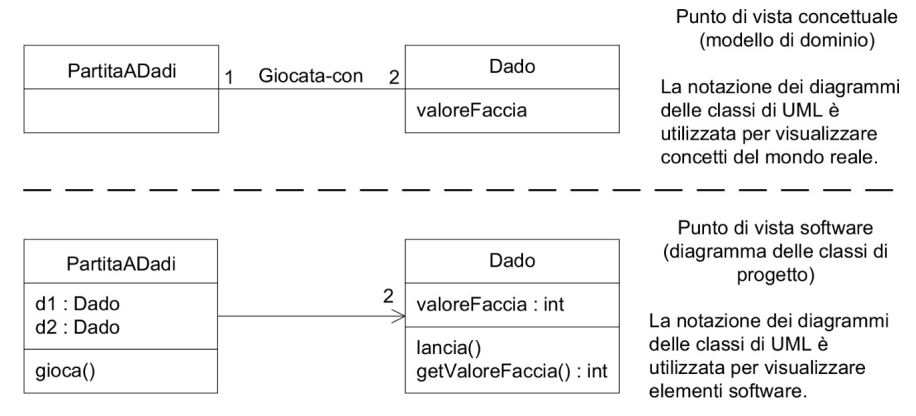
\includegraphics[width = 0.80\textwidth]{Images/11.PNG}
\end{center}
Quindi, in pratica, UMl viene usato:
\begin{enumerate}
    \item \textbf{Nell'analisi}, principalmente secondo il \textbf{punto di vista concettuale}
    \item \textbf{Nella progettazione}, principalmente secondo il \textbf{punto di vista software}
\end{enumerate}
\subsubsection{Significato di classe}
Nell'UML grezzo, abbiamo chiamato "classi" un insieme di oggetti; ma questo termine racchiude una \textbf{varietà di casi}: oggetti fisici, concetti astratti, elementi software, eventi e così via.
In particolare, una classe UML è un caso particolare di un modello UML generale chiamato \textbf{classificatore}, che è qualcosa che ha delle caratteristiche strutturali e/o comportamentali e comprende \textbf{classi, attori, interfacce e casi d'uso}.
Un metodo \textbf{impone una terminologia alternativa sovrapposta all'UML grezzo}; in particolare, ci adegueremo a quella di \textbf{UP} (Unified Process), che chiama:
\begin{itemize}
    \item \textbf{Classe concettuale}: Oggetto o concetto \textbf{del mondo reale} da un punto di vista \textbf{concettuale}. Il modello di dominio di UP contiene \textbf{classi concettuali}
    \item \textbf{Classi software}: Una classe che rappresenta un \textbf{componente software}, da un punto di vista \textbf{software}, indipendentemente dal processo, metodo o linguaggio di programmazione. Il modello di progetto di UP contiene \textbf{classi software}.
\end{itemize}
\subsubsection{Vantaggi della modellazione visuale}
Disegnare e leggere UML implica che si sta lavorando in \textbf{modo visuale}. La modellazione visuale ci permette di sfruttare le capacità del nostro cervello di \textbf{comprendere rapidamente simboli, unità e relazioni nelle notazioni} (prevalentemente bidimensionali) a "rettangoli e linee".
I diagrammi ci aiutano a vedere o esaminare meglio il \textbf{quadro generale} e le relazione tra elementi dell'analisi del software e allo stesso tempo ci permettono di \textbf{ignorare o nascondere i dettagli poco interessanti}.
\section{Processi per lo sviluppo del software}
Un \textbf{processo per lo sviluppo del software} (o \textbf{processo software}) definisce un approccio disciplinato per la \textbf{costruzione}, il \textbf{rilascio} e la \textbf{manutenzione del software}.
Definisce quindi \textbf{chi fa che cosa, quando e come} per raggiungere un certo obbiettivo. In particolare:
\begin{itemize}
    \item \textbf{Cosa} sono le \textbf{attività}
    \item \textbf{Chi} sono i \textbf{ruoli}
    \item \textbf{Come} sono le \textbf{metodologie}
    \item \textbf{Quando} riguarda \textbf{l'organizzazione temporale} delle attività
\end{itemize} 
\newpage
\noindent
Le attività fondamentali di un processo di sviluppo sono:
\begin{center}
    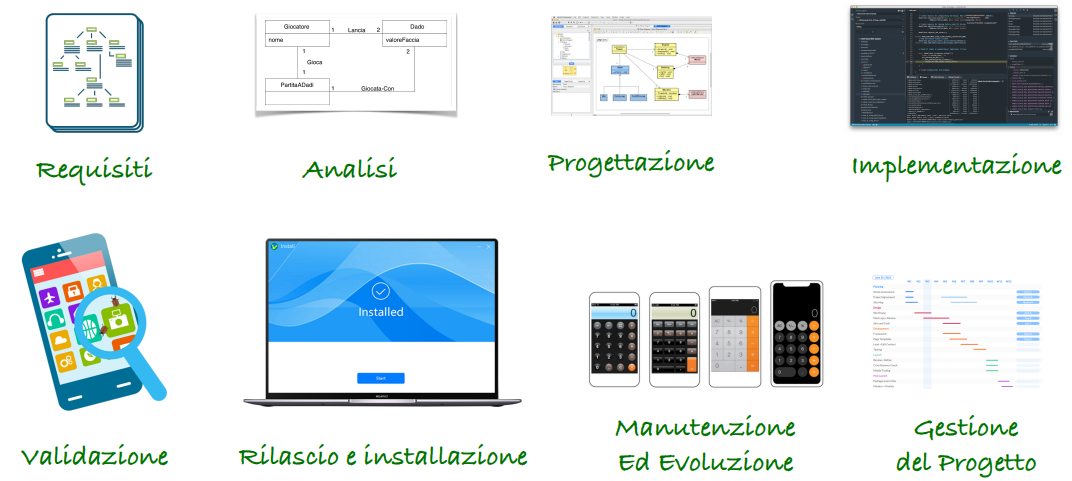
\includegraphics[width = 1\textwidth]{Images/12.PNG}
\end{center}
Ciò che distingue i processi software gli uni dagli altri è tuttavia \textbf{sono le scelte che riguardano l'organizzazione temporale delle attività} (quando), ovvero il modo in cui essi rispondono alle domande:
\begin{itemize}
    \item Per quanto tempo continueremo a svolgere questa attività
    \item Cosa faremo dopo?
\end{itemize}
\subsection{Processi agili e basati sul piano}
I processi \textbf{orientati al piano} sono processi in cui tutte le attività sono \textbf{pianificate in anticipo} e i progressi del progetto sono \textbf{misurati rispetto a questo piano}.
Invece, nei \textbf{processi agili}, la pianificazione è \textbf{incrementale}, quindi risulta più facile modificare il processo per riflettere le mutevoli esigenze del cliente.
In pratica, \textbf{la maggior parte dei processi software include elementi di entrambi gli approcci}. È necessario notare che \textbf{non esistono processi software totalmente sbagliati o corretti}.
\subsection{Modelli di processo software}
In pratica, la maggior parte dei sistemi di grandi dimensioni vengono sviluppati usando processi che incorporano elementi dei seguenti modelli:
\begin{itemize}
    \item \textbf{Sviluppo a cascata}: Modello \textbf{basato sul piano}. Fasi separate di \textbf{specifica} e di \textbf{sviluppo}
    \item \textbf{Sviluppo incrementale}: \textbf{Specifica, sviluppo e validazione} si alternano. Può essere guidato dal piano o agile
    \item \textbf{Integrazione e configurazione}: Il sistema viene assemblato a partire da \textbf{componenti esistenti e configurabili}. Può essere basato sul piano o agile
\end{itemize} 
Tuttavia "\textbf{quale scegliere?}" è una domanda assolutamente non banale. Diamo quindi dei motivi per il quale esistono diversi processi software:
\begin{itemize}
    \item \textbf{Complessità del progetto}: I progetti software possono variare \textbf{in termini di complessità}, da semplici applicazioni a sistemi complessi e "mission-critical".
    La complessità di un progetto \textbf{influenza il livello di formalismo e struttura} necessari nel processo di sviluppo
    \item \textbf{Dimensione del team}: Il numero di persone che lavorano ad un progetto software \textbf{influenza come il lavoro viene organizzato e coordinato}.
    Team di grandi dimensioni avranno quindi bisogno di \textbf{un processo più formale} rispetto a team di piccole dimensioni
    \item \textbf{Budget e tempistiche}:  Il budget e le tempistiche di un progetto software \textbf{influenzano il modo in cui il progetto viene organizzato e gestito}.
    Progetti software con \textbf{budget e tempistiche limitate} avranno bisogno di un processo software \textbf{più snello} rispetto a progetti con budget e tempistiche flessibili
    \item \textbf{Rischio}: Il \textbf{rischio} associato ad un progetto software influenza il \textbf{livello di rigore e controllo} necessari nel processo di sviluppo.
    Maggiore è il fattore di rischio, maggiore sarà il \textbf{rigore} che il processo software dovrà avere.
\end{itemize}
\subsubsection{Integrazione e configurazione}
Questo modello è basato sul \textbf{riutilizzo del software}, in cui i sistemi sono \textbf{integrati da componenti o sistemi applicativi esistenti} (talvolta chiamati \textbf{sistemi COTS}: \textit{commercial-off-the-shelf}).
Gli elementi riutilizzati possono essere \textbf{configurati} in modo da adattarli alle esigenze del cliente. Il riutilizzo è oggi il sistema standard per la costruzione di molti tipi di software aziendali. \newline
Quali sono però i tipi di "software riutilizzabile"?
\begin{itemize}
    \item Sistemi applicativi \textbf{stand-alone} (COTS) configurati per l'uso in un particolare ambiente
    \item \textbf{Collezioni di oggetti} sviluppate come \textbf{pacchetti} da integrare con un \textbf{framework} di componenti (es. .NET o J2EE)
    \item \textbf{Servizi web} sviluppati secondo lo \textbf{standard di servizio} e invocabili in maniera remota
\end{itemize}
L'intero processo quindi \textbf{definisce un'ingegneria del software orientata al riuso}:
\begin{center}
    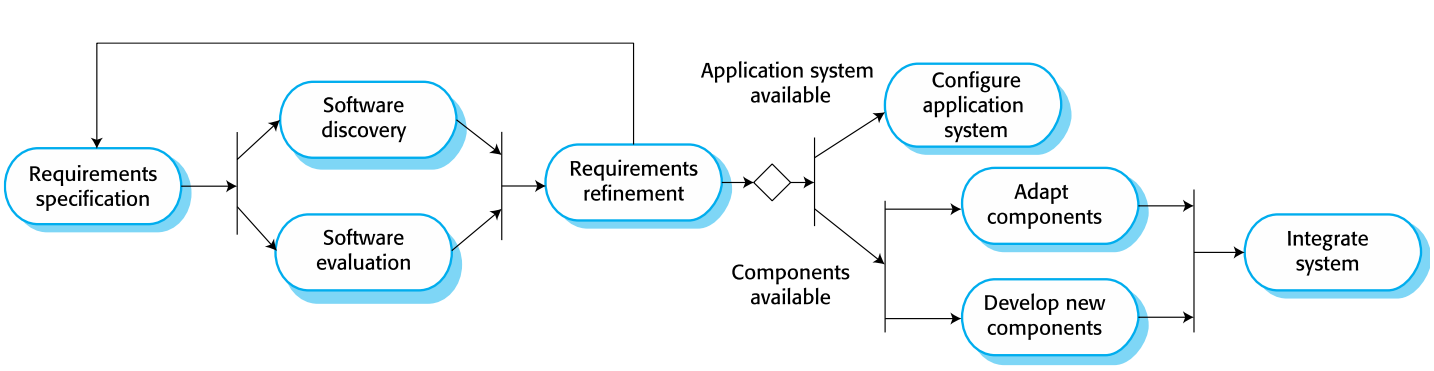
\includegraphics[width = 1.10\textwidth]{Images/13.png}
\end{center}
\newpage
\noindent
Vediamo ora i vantaggi e gli svantaggi di questo approccio:
\begin{itemize}
    \item \textbf{Vantaggio}: Riduzione dei costi e dei rischi, poiché \textbf{viene sviluppato meno software da zero}
    \item \textbf{Vantaggio}: Consegna più rapida del sistema al cliente
    \item \textbf{Svantaggio}: Si dovranno attuare dei \textbf{compromessi sui requisiti}, quindi il sistema potrebbe non soddisfare appieno le esigenze dell'utente
    \item \textbf{Svantaggio}: Perdita di controllo sull'\textbf{evoluzione} delle varie componenti che formano il sistema
\end{itemize}
\subsubsection{Processo a cascata}
\begin{center}
    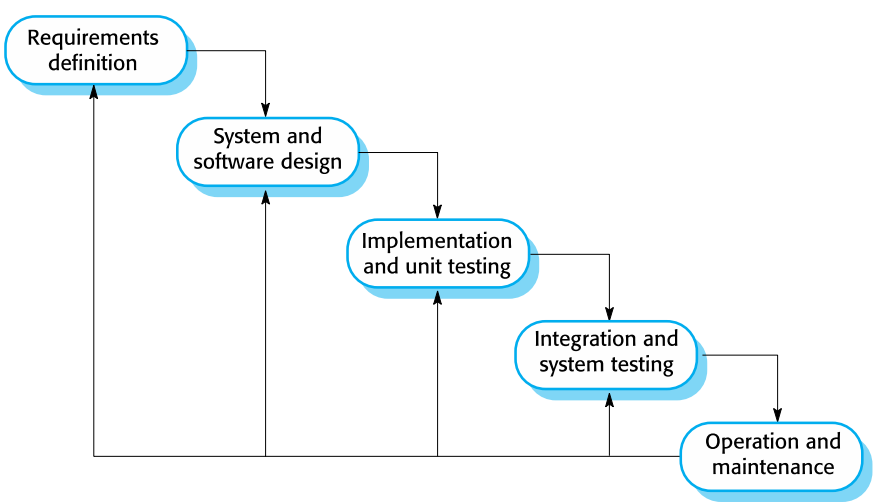
\includegraphics[width = 0.80\textwidth]{Images/14.png}
\end{center}
Il processo a cascata è il processo software \textbf{più vecchio} tra quelli utilizzati ancora oggi.
Il processo software con ciclo di vita a cascata (o \textbf{sequenziale}) è, in prima approssimazione, basato su uno svolgimento \textbf{sequenziale delle diverse attività di sviluppo del software}.
All'inizio di un progetto, vengono definiti in dettaglio \textbf{tutti i requisiti} (o almeno la maggior parte di essi); allo stesso modo, più o meno all'inizio del progetto, si cerca di stabilire un \textbf{piano temporale dettagliato e "affidabile"} delle attività da svolgere (non è detto che lo sia).
Poi si prosegue con la \textbf{modellazione} (analisi e progettazione) e viene creato un \textbf{progetto completo del software}. Solo a questo punto inizia la \textbf{programmazione del sistema software}, a cui seguiranno \textbf{verifica, rilascio e manutenzione}. Si noti come \textbf{ogni fase descritta inizia solo quando la precedente finisce}.
Ad essere precisi, il processo a cascata \textbf{permette la possibilità di feedback e cicli tra le attività}, ma la maggior parte delle organizzazioni che applica questo processo considera di solito una \textbf{sequenzialità stretta} fra le varie fasi.
Il principale svantaggio del processo a cascata è quindi quello di \textbf{avere difficoltà ad accogliere i cambiamenti a processo avviato}.
Il processo a cascata, tuttavia, \textbf{risulta una pratica mediocre per la maggior parte dei progetti software} ([Larman03] e [LB03]): infatti il processo a cascata è associato ad una \textbf{percentuale elevata di fallimenti}. Perché quindi questo processo è così soggetto a frequenti fallimenti?
\begin{itemize}
    \item La suddivisione \textbf{inflessibile} del progetti in \textbf{fasi distinte} rende difficile rispondere alle mutevoli esigenze di un cliente
    \begin{itemize}
        \item Pertanto, questo modello è appropriato \textbf{solo quando i requisiti sono ben compresi e le modifiche saranno piuttosto limitate durante il processi di sviluppo}. Questo però non accade, come mostrato dal seguente grafico dello studio [Jones97]:
        \begin{center}
            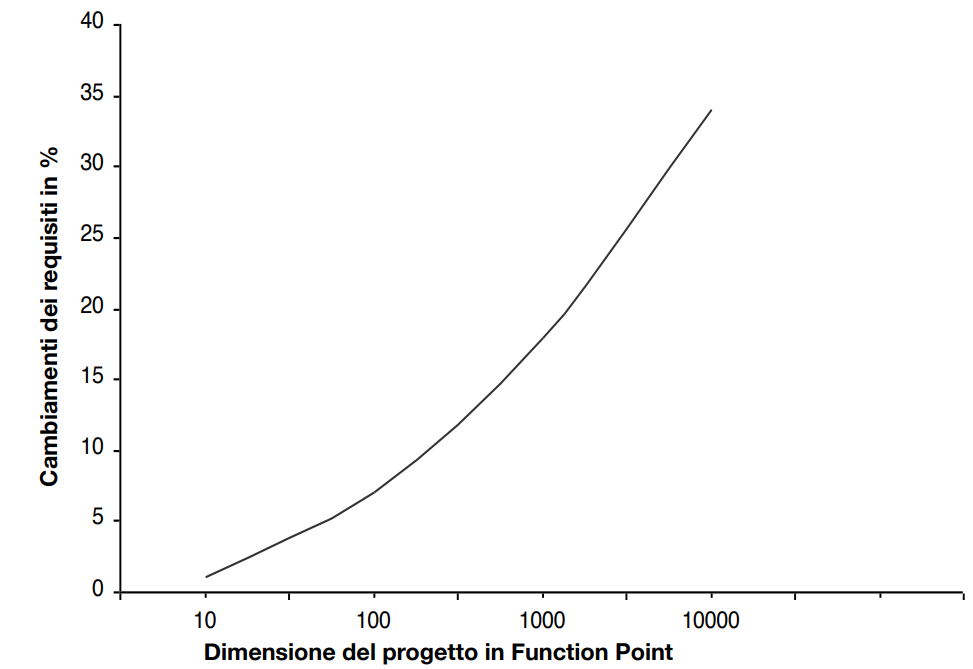
\includegraphics[width = 0.70\textwidth]{Images/15.png}
        \end{center}
    \end{itemize}
    \item Il modello a cascata viene utilizzato principalmente per progetti di \textbf{ingegneria dei sistemi di grandi dimensioni}, in cui un sistema viene sviluppato in diversi siti.
    \begin{itemize}
        \item In questo caso, la natura pianificata del processo a cascata \textbf{aiuta a coordinare il lavoro}
    \end{itemize}
\end{itemize}
\subsubsection{Sviluppo iterativo, incrementale ed evolutivo}
Una pratica fondamentale di molti processi software moderni (come UP e SCRUM) è lo \textbf{sviluppo iterativo}.
In questo approccio al ciclo di vita, lo sviluppo è suddiviso in \textbf{una serie di mini progetti} dalla durata temporale fissa (es. 3 settimane, si dicono quindi \textbf{timeboxed}) chiamate \textbf{iterazioni};
il risultato di ciascuna iterazione è \textbf{un sistema eseguibile, testato e integrato, ma parziale}. Ciascuna iterazione prevede le proprie fasi di \textbf{analisi dei requisiti, progettazione, implementazione e test}.
Il ciclo di vita iterativo si basa sul \textbf{susseguirsi di ampliamenti e raffinamenti} di un sistema nel corso di \textbf{molteplici iterazioni}, con \textbf{feedback e adattamenti ciclici} come guide essenziali per \textbf{convergere verso un sistema appropriato}.
Il sistema quindi \textbf{cresce in modo incrementale} nel tempo. Poiché il feedback e l'adattamento fanno \textbf{evolvere il sistema nel tempo}, questo processo si dice anche \textbf{evolutivo}.
\begin{center}
    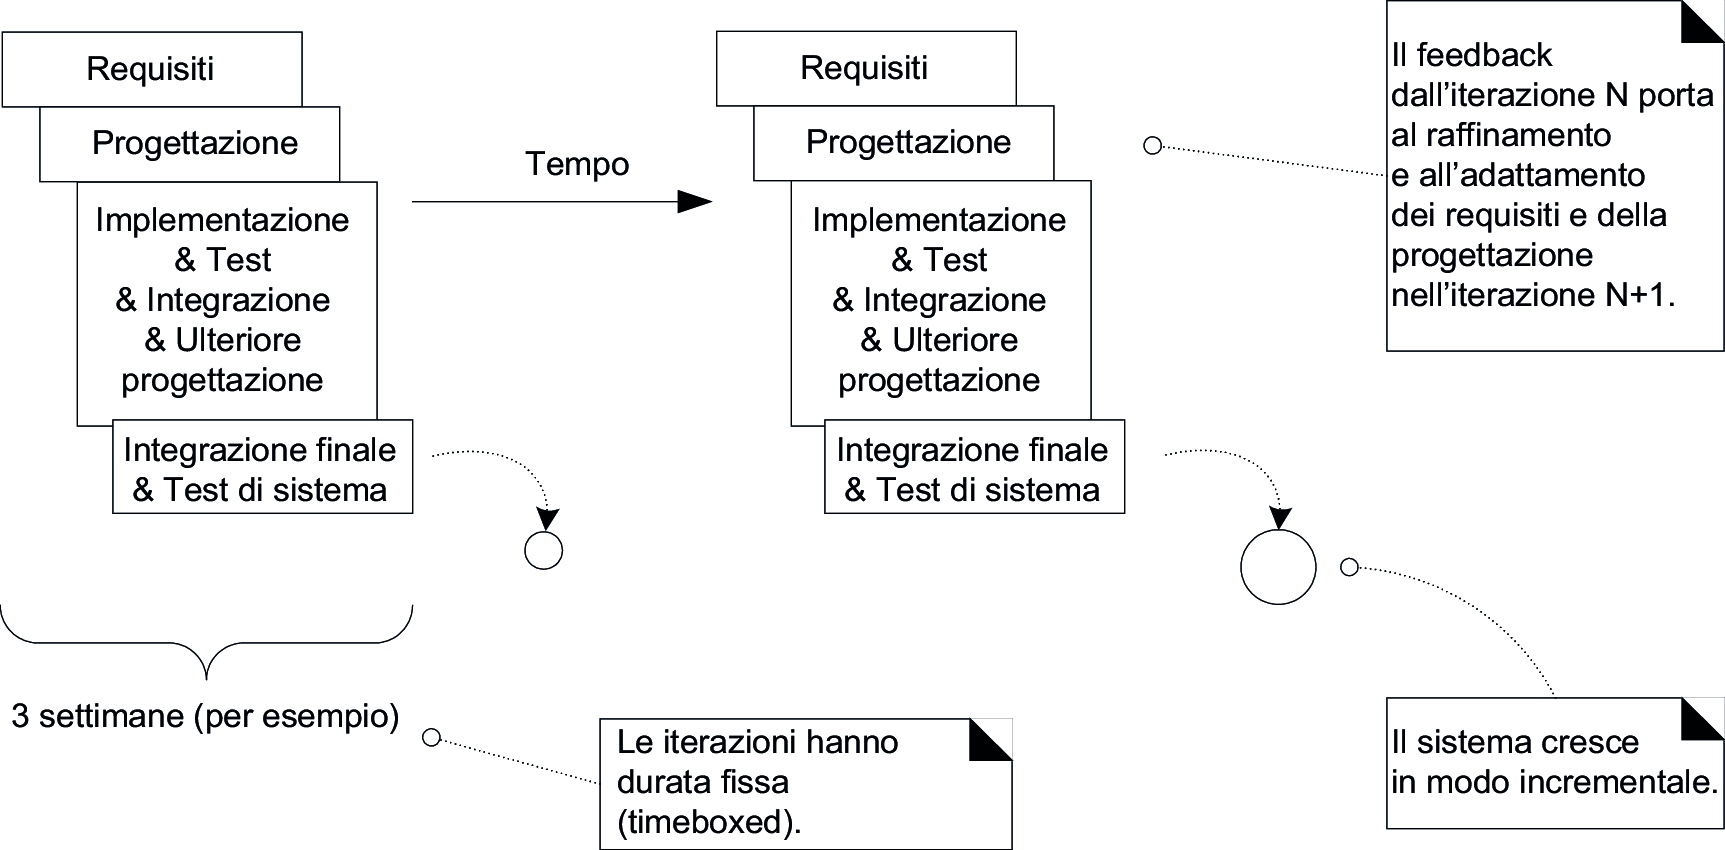
\includegraphics[width = 1\textwidth]{Images/16.png}
\end{center}
Quindi lo sviluppo iterativo, incrementale ed evolutivo si basa su un atteggiamento di \textbf{accettazione del cambiamento} e sull'\textbf{adattamento} come guide \textbf{inevitabili e di fatto essenziali}.
Tuttavia questo non significa che questo processo supporti uno sviluppo \textbf{caotico} e che gli sviluppatori continuino a cambiare direzione in base alle richieste estemporanee del cliente ("feature creep"). Una via di
mezzo \textbf{è possibile}:
\begin{itemize}
    \item Ciascuna iterazione comporta la scelta di un \textbf{di un piccolo sottoinsieme di requisiti, una rapida progettazione, implementazione e test}.
    Seppur nelle iterazioni iniziali ciò che si produce \textbf{sarà lontano da ciò che si vuole ottenere}, ciò permette al cliente di dare feedback in maniera \textbf{rapida e precoce}; i quali potranno essere \textbf{analizzati dal team di lavoro} per ottenere delle \textbf{indicazioni pratiche e significative}; ciò permette al team anche di avere un'opportunità di \textbf{modificare o adattare la comprensione dei requisiti e il progetto}.
    Oltre al chiarimento dei requisiti, attività quali i \textbf{test di carico} dimostreranno se il progetto e l'implementazione parziale sono nella direzione giusta o se è necessaria una modifica dell'architettura.
    \item Il lavoro procede mediante una serie di \textbf{cicli strutturati di costruzione-feedback-adattamento}
    \item Nel tempo, attraverso il \textbf{feedback iterativo} e \textbf{l'adattamento}, il sistema sviluppato \textbf{evolve} e \textbf{converge} verso i requisiti corretti e il progetto più appropriato
    \begin{itemize}
        \item Non bisogna stupirsi se nelle prime iterazioni lo \textbf{scostamento} dal sistema desiderato è maggiore che in quelle successive
        \item L'instabilità dei requisiti e del progetto \textbf{tende a diminuire nel tempo}, tuttavia nelle iterazioni finali è \textbf{difficile ma non impossibile} che si verifichi un \textbf{cambiamento significativo dei requisiti}
    \end{itemize}
\end{itemize}
Quali sono quindi i \textbf{vantaggi} dello sviluppo iterativo, incrementale ed evolutivo?
\begin{itemize}
    \item \textbf{Minore probabilità di fallimento del progetto}, \textbf{migliore produttività}, \textbf{percentuali più basse di difetti}
    \item Riduzione precoce, anziché tardiva, dei \textbf{rischi maggiori} (tecnici, requisiti obbiettivi ecc...)
    \item Progresso visibile \textbf{sin dall'inizio}
    \item \textbf{Feedback precoce}, coinvolgimento dell'utente e adattamento, che portano a un sistema che soddisfa al meglio le esigenze reali delle parti interessate
    \item \textbf{Gestione della complessità}, cioè il team non viene sopraffatto dalla "\textbf{paralisi da analisi}" o da \textbf{passi molto lunghi e complessi}
    \item Ciò che si apprende nel corso di un iterazione \textbf{può essere usato per migliorare le successive}
\end{itemize}
Tuttavia questo processo \textbf{non è privo di svantaggi}:
\begin{itemize}
    \item Il processo \textbf{non è visibile}: i manager hanno bisogno di documenti \textbf{costanti} per tenere traccia del processo di sviluppo; tuttavia se il sistema continua a cambiare non è conveniente continuare a produrre documenti che riflettono ogni versione del sistema
    \item La struttura del sistema \textbf{tende a degradarsi} con l'aggiunta di nuovi incrementi: a meno che non si dedichi tempo e denaro al \textbf{refactoring} per migliorare il software, le aggiunte tendono a \textbf{corrompere la struttura del sistema}; quindi incorporare sempre più modifiche software diventa sempre più \textbf{difficile e costoso}
\end{itemize}
Lo sviluppo iterativo è basato sul fatto che nei sistemi complessi e mutevoli, il feedback e l'adattamento sono \textbf{incrementi chiave} per il successo:
\begin{itemize}
    \item Feedback proveniente dalle \textbf{attività iniziali di sviluppo}, dai \textbf{programmatori} che cercano di leggere le specifiche e da \textbf{dimostrazioni ai clienti} per raffinare i requisiti
    \item Feedback proveniente dai \textbf{test} e dagli \textbf{sviluppatori} che raffinano il progetto e i modelli
    \item Feedback circa \textbf{l'avanzamento del team} nell'affrontare le prime caratteristiche, per raffinare le \textbf{stime di tempo e di costi}
    \item Feedback proveniente dal \textbf{cliente e dal mercato} per assegnare/modificare le \textbf{priorità} alle caratteristiche da affrontare nell'iterazione successiva
\end{itemize}
Una pratica fondamentale dello sviluppo iterativo è quella di avere \textbf{iterazioni di lunghezza fissata}, cioè \textbf{timeboxed}; il periodo consigliato è dalle \textbf{due alle sei settimane}.
Iterazioni più lunghe sono invece contrarie allo spirito dello sviluppo iterativo, poiché esso richiede \textbf{un feedback costante da parte del cliente}; con un periodo più lungo di sei settimane la complessità \textbf{cresce} e il feedback viene \textbf{ritardato}.
Iterazioni più corte di due settimane invece \textbf{difficilmente permettono di sviluppare abbastanza software} per avere un feedback significativo.
In questo processo di sviluppo \textbf{non è consentito ritardare la fine di un'iterazione}: se risulta difficile portare a termine tutti i requisiti che si erano previsti per una particolare iterazione, è meglio \textbf{spostarli all'iterazione successiva} piuttosto che modificare la durata dell'iterazione.
Un'iterazione di durata fissa è detta \textbf{timeboxed}. \newline
Bisogna anche fare attenzione che il \textbf{pensiero a cascata non si infiltri nello sviluppo iterativo}; segni di questa infiltrazione sono:
\begin{itemize}
    \item Si è scritto \textbf{la maggior parte dei requisiti o dei casi d'uso} prima dello sviluppo
    \item Si è creato in modo \textbf{dettagliato e completo delle specifiche, dei modelli o il progetto} prima di iniziare l'implementazione 
\end{itemize}
L'adozione dello sviluppo iterativo richiede che il software venga realizzato in modo \textbf{flessibile}, affinche l'impatto dei cambiamenti sia \textbf{il più basso possibile}. A tal fine il codice (e il progetto del software) devono essere \textbf{facilmente modificabili}.
Per facilitare questo aspetto il codice deve essere quindi \textbf{leggibile e facilmente comprensibile}, la mancanza di questa qualità infatti rende difficile implementare i cambiamenti in modo incrementale; inoltre è necessario usare degli \textbf{strumenti metodologici opportuni}; per esempio \textbf{tecnologie ad oggetti, sviluppo guidato dai test e refactoring}.
Vediamo un esempio visuale sul come avviene uno sviluppo iterativo, incrementale ed evolutivo se assumiamo 20 iterazioni (assumiamo di star seguendo UP):
\begin{center}
    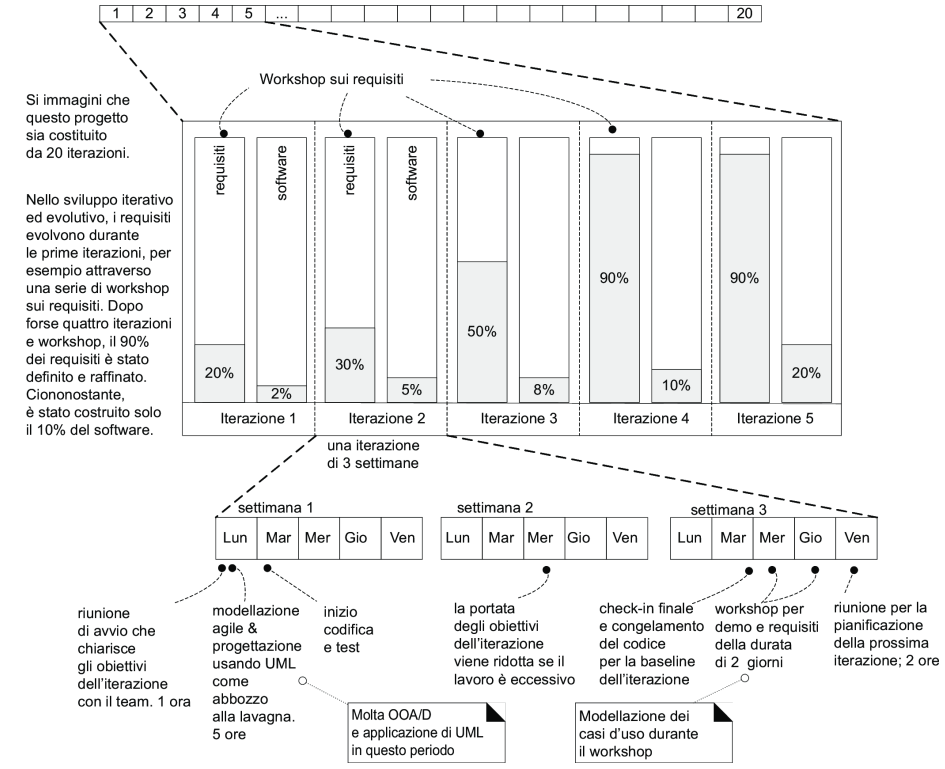
\includegraphics[width = 1\textwidth]{Images/17.png}
\end{center}
Un'attività critica dello sviluppo iterativo è la \textbf{pianificazione delle iterazioni}, cioè la definizione delle \textbf{attività da svolgere in ogni iterazione}.
Se si sta seguendo un processo iterativo, è necessario evitare di \textbf{tentare di pianificare l'intero progetto in modo dettagliato sin dalla prima iterazione}.
Piuttosto, i processi iterativi promuovono una \textbf{pianificazione iterativa} (o adattiva), in cui in ciascuna iterazione viene stabilito il \textbf{piano di lavoro dettagliato di una singola iterazione}.
In UP, la pianificazione viene effettuata alla \textbf{fine dell'iterazione corrente} per decidere le attività della \textbf{seguente iterazione}. In SCRUM, la pianificazione viene effettuata \textbf{all'inizio dell'iterazione} per stabilire il piano dell'iterazione \textbf{corrente}.
Lo sviluppo iterativo promuove la pianificazione \textbf{guidata dal rischio e guidata dall'utente}.
Ciò significa che gli obbiettivi delle iterazioni iniziali vengono scelti
\begin{enumerate}
    \item Per \textbf{identificare e attenuare i rischi maggiori}
    \item Per \textbf{costruire e rendere visibili} le caratteristiche a cui il cliente tiene di più
\end{enumerate}
In particolare, la progettazione guidata dal rischio contiene in sè la pratica dello \textbf{sviluppo centrato sull'architettura}: le prime iterazioni si concentreranno sulla \textbf{costruzione, test e la stabilizzazione del nucleo dell'architettura}.
Infatti, è un rischio molto alto \textbf{non avere un'architettura di base solida}. \newline
Importante per il processo iterativo è il \textbf{non cambiare gli obbiettivi dell'iterazione}: durante ciascuna iterazione, i requisiti su cui operare \textbf{vengono prima fissati} (pianificazione iterativa) e poi \textbf{bloccati}, cioè non sono più modificabili.
Durante ciascuna iterazione, quindi, il team \textbf{può lavorare al suo meglio}, poiché:
\begin{itemize}
    \item I requisiti sono \textbf{bloccati}, quindi il team non può essere \textbf{nè interrotto ne disturbato durante l'iterazione}
    \item I committenti possono interagire con il team di sviluppo \textbf{solo alla fine dell'iterazione}
\end{itemize}
Durante un'iterazione è tuttavia possibile che il team di sviluppo decida di \textbf{cambiare il piano dell'iterazione}, per esempio quando valuta, a metà dell'iterazione, la possibilità di raggiungere gli obbiettivi prefissati nella durata prevista.
\section{Unified Process (UP)}
Il \textbf{processo unificato} (unified process) o \textbf{UP} è un processo iterativo diffuso per lo sviluppo software orientato agli oggetti.
UP è molto \textbf{flessibile e aperto}: incoraggia infatti l'uso di \textbf{altre pratiche} prese da \textbf{altri processi iterativi}, come SCRUM o Extreme Programming.
UP è:
\begin{itemize}
    \item \textbf{Pilotato dai casi d'uso} (requisiti) e dai \textbf{fattori di rischio}
    \item Incentrato \textbf{sull'architettura}
    \item \textbf{Iterativo, incrementale ed evolutivo}
\end{itemize}
L'idea principale da apprezzare e praticare in UP è lo \textbf{sviluppo iterativo, evolutivo e incrementale} con \textbf{timeboxing breve}. Ulteriori best practices e concetti chiavi di UP sono:
\begin{itemize}
    \item Affrontare le problematiche di \textbf{rischio maggiore} e valore elevato nelle \textbf{iterazioni iniziali}
    \item Impegnare gli utenti \textbf{continuamente} sulla valutazione, il feedback e i requisiti
    \item Creare un'architettura \textbf{coesa} nelle iterazioni iniziali
    \item Verificare continuamente le \textbf{qualità}: testare \textbf{spesso, presto e in modo realistico}
    \item Applicare i \textbf{casi d'uso}, se appropriato
    \item Fare della \textbf{modellazione visuale} (con UML)
    \item Gestire attentamente i requisiti
    \item Gestire le richieste di cambiamento e le configurazione
\end{itemize}
Vediamo una sua breve storia:
\begin{center}
    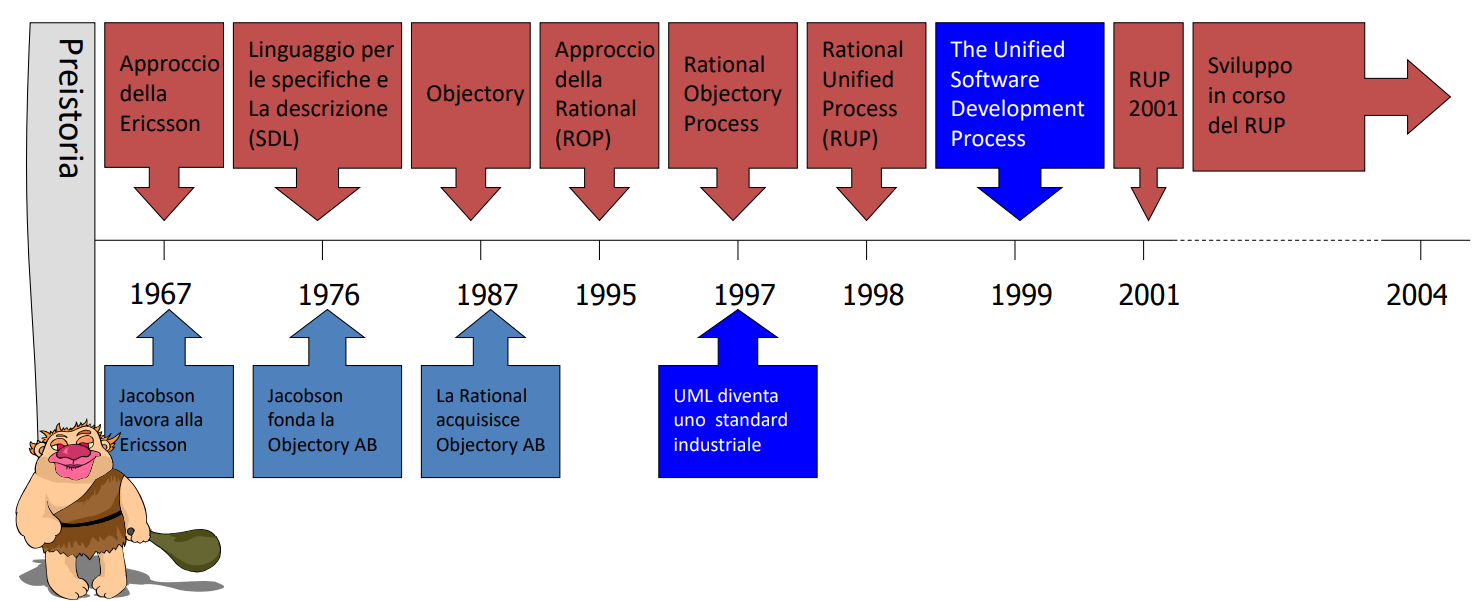
\includegraphics[width = 1\textwidth]{Images/18.png}
\end{center}
\subsection{Iterazioni e discipline}
Le iterazioni sono \textbf{concetti chiave} in UP. Esse sono come un mini-progetto che include:
\begin{itemize}
    \item \textbf{Pianificazione}
    \item \textbf{Analisi e progettazione}
    \item \textbf{Costruzione}
    \item \textbf{Integrazione e test}
    \item \textbf{Un rilascio}
\end{itemize}
Poiché UP è un processo iterativo, si arriva al \textbf{rilascio finale} dopo una \textbf{serie di iterazioni}. 
Le iterazioni \textbf{possono sovrapporsi}; ciò permette lo \textbf{sviluppo parallelo e il lavoro flessibile in grandi squadre}.
Tuttavia richiede un'attenta pianificazione. \newline
UP colloca le attività lavorative in \textbf{discipline}; una disciplina è \textbf{un insieme di attività e dei relativi elaborati in una determinata area}, come, per esempio, l'area dell'analisi dei requisiti.
In UP, un \textbf{elaborato} è il termine generico con cui si fa riferimento ad un qualsiasi \textbf{prodotto di lavoro} (codice, schema di basi di dati, ecc...).
UP definisce diverse discipline ed elaborati, ma noi ci concentreremo su:
\begin{itemize}
    \item \textbf{Modellazione di business}: L'elaborato \textbf{Modello di dominio}, per visualizzare i concetti significativi nel dominio di applicazione
    \item \textbf{Requisiti}: Gli elaborati \textbf{Modello dei casi d'uso e Specifica supplementare}, per descrivere i \textbf{requisiti funzionali e non funzionali}
    \item \textbf{Progettazione}: L'elaborato \textbf{Modello di progetto}, per il progetto degli oggetti software
\end{itemize}
Un elenco più ampio è il seguente:
\begin{center}
    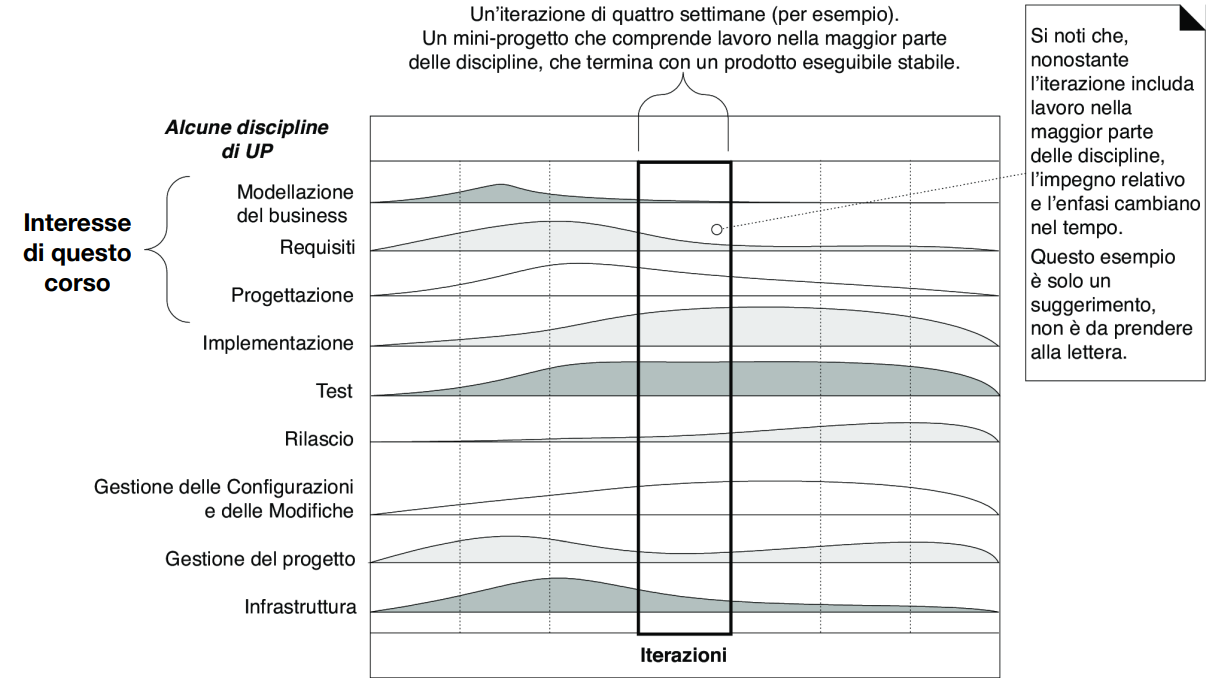
\includegraphics[width = 1.10\textwidth]{Images/19.png}
\end{center}
Come si può vedere sopra, anche se ogni iterazione può prevedere \textbf{tutti i flussi di lavoro}, la collocazione dell'iterazione all'interno del ciclo di vita del progetto \textbf{determina una maggiore enfasi} su uno dei flussi di lavoro.
\subsubsection{Release}
Ogni iterazione \textbf{genera una release}: una release è un \textbf{insieme di manufatti}, previsti e approvati. Essa fornisce una \textbf{base approvata per le successive attività di analisi e sviluppo}.
Un \textbf{incremento} è la \textbf{differenza} tra una release e la successiva. Costituisce quindi un passo in avanti verso il rilascio finale del sistema.
\newpage
\subsection{Fasi di UP}
Un progetto UP organizza il lavoro in quattro \textbf{fasi temporali principali e successive}:
\begin{enumerate}
    \item \textbf{Ideazione}: Visione \textbf{approssimativa}, studio economico, porta, stime \textbf{approssimative} dei costi e dei tempi
    \item \textbf{Elaborazione}: Visione \textbf{raffinata}, implementazione \textbf{iterativa} del \textbf{nucleo dell'architettura}, risoluzione dei rischi maggiori, identificazione della \textbf{maggior parte} dei requisiti, stime più realistiche.
    \item \textbf{Costruzione}: Implementazione \textbf{iterativa} degli elementi rimanenti, più facili e a rischio minore; preparazione al rilascio
    \item \textbf{Transizione}: beta test, rilascio finale
\end{enumerate}
Si noti che questo modello \textbf{non è a cascata}: l'ideazione \textbf{non è una fase di requisiti}; piuttosto è una breve fase di \textbf{fattibilità} in cui viene eseguita un'indagine \textbf{sufficiente} a sostenere la decisione di continuare o interrompere il progetto.
Allo stesso modo, la fase di \textbf{elaborazione} non è una fase dei requisiti o dell'implementazione; piuttosto è una fase in cui \textbf{viene implementato il nucleo dell'architettura} e si risolvono i rischi maggiori.
Vediamo un'esempio visuale:
\begin{center}
    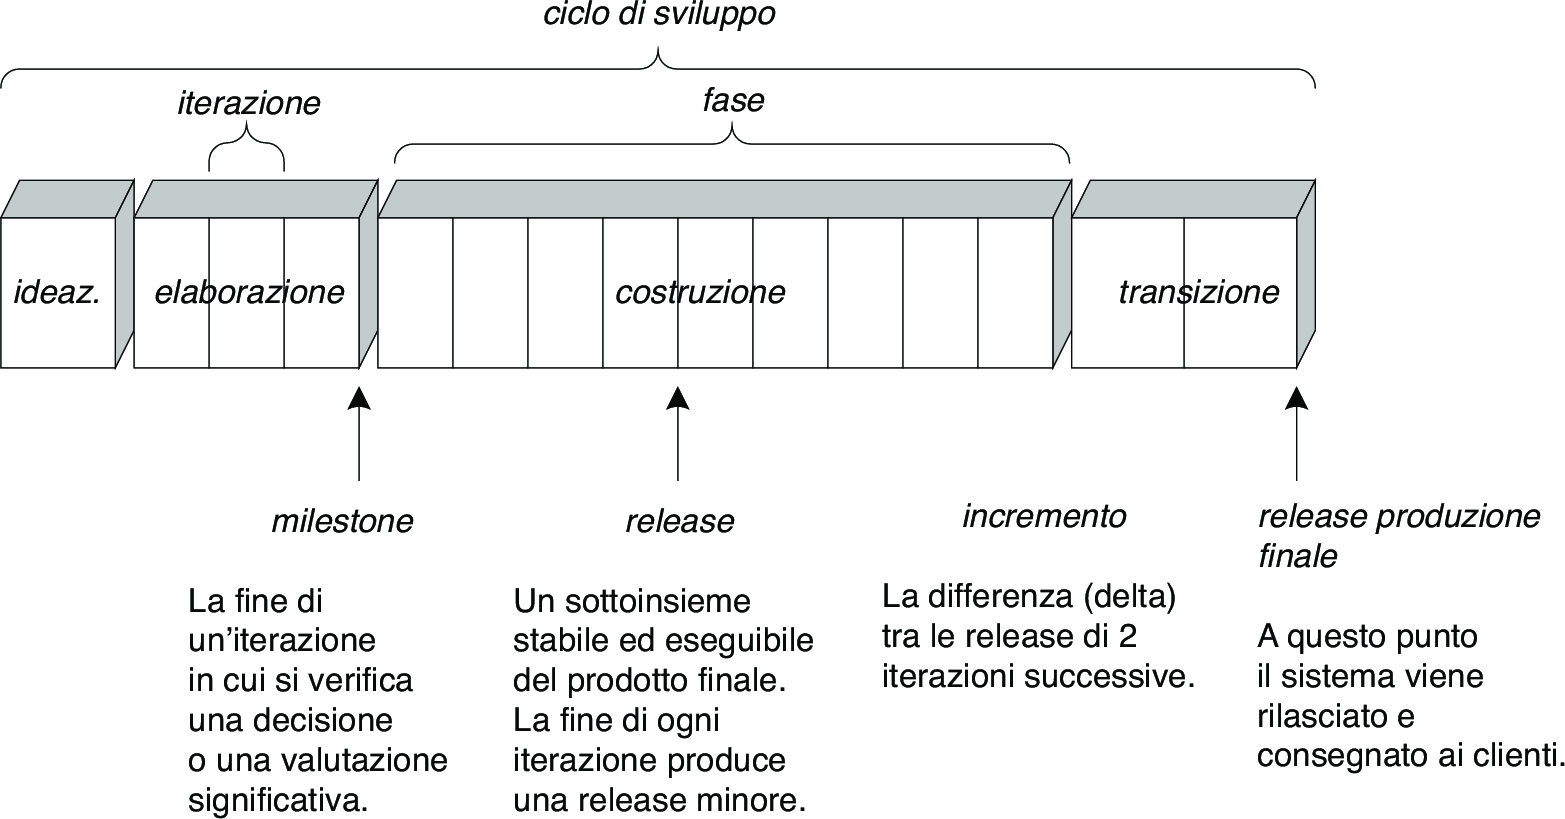
\includegraphics[width = 1\textwidth]{Images/20.png}
\end{center}
\begin{center}
    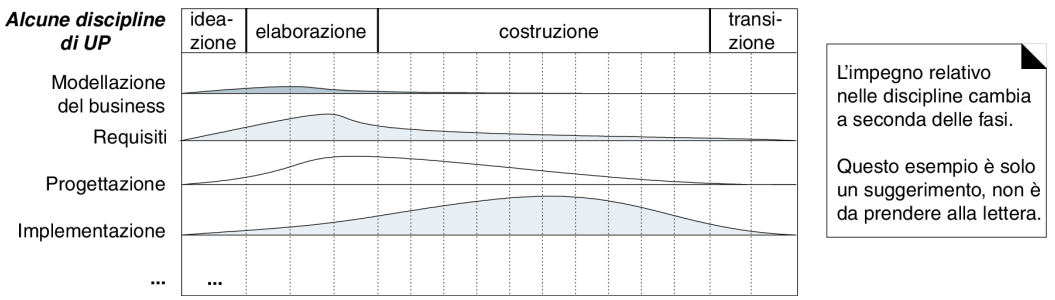
\includegraphics[width = 1\textwidth]{Images/21.png}
\end{center}
\subsection{Scenari di sviluppo di UP}
Tra gli elaborati e le pratiche di UP, \textbf{quasi tutto è opzionale}
\begin{itemize}
    \item Alcune pratiche e principi di UP \textbf{sono fissi}, come lo \textbf{sviluppo iterativo e guidato dal rischio} e \textbf{il controllo continuo della qualità}
    \item Tutte le attività e gli elaborati sono \textbf{opzionali}, con l'ovvia esclusione del codice
\end{itemize}
La scelta delle pratiche degli elaborati UP per un progetto può essere scritta in un breve documento chiamato \textbf{scenario di sviluppo}
\begin{center}
    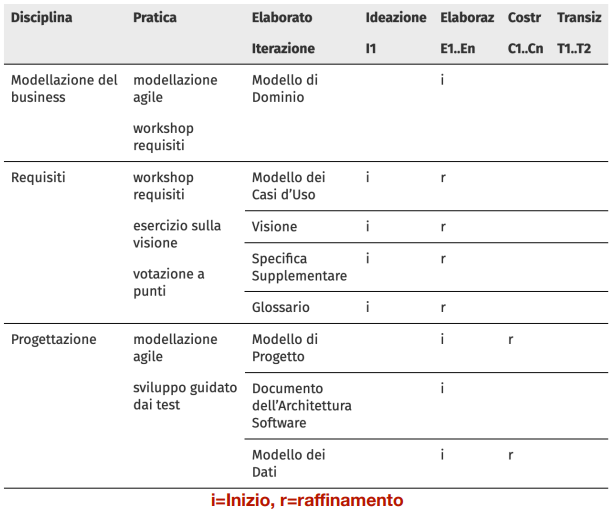
\includegraphics[width = 0.90\textwidth]{Images/22.png}
\end{center}
\section{Metodologie e processi agili}
Lo sviluppo agile è una forma di \textbf{sviluppo iterativo} che incoraggia \textit{l'agilità}, ovvero una risposta \textbf{rapida e flessibile} ai cambiamenti.
Le pratiche agili, come \textbf{Agile Modelling}, sono fondamentali per applicare UML correttamente.
I metodi di sviluppo agile di solito applicano lo sviluppo \textbf{iterativo ed evolutivo}, con iterazioni brevi e timeboxed, fanno uso della \textbf{pianificazione iterativa}, promuovono le \textbf{consegne incrementali} e comprendono altri valori che incoraggiano l'agilità.
Non è possibile dare una definizione di "\textbf{metodo agile}", poiché le pratiche adottate variano da metodo a metodo. Tuttavia una pratica di base, adottata da tutti i metodi, è quella che prevede \textbf{iterazioni brevi}, con un \textbf{raffinamento evolutivo dei piani, dei requisiti e del progetto}.
Inoltre, essi promuovono pratiche e principi che riflettono una \textbf{sensibilità agile} per \textbf{la semplicità, la leggerezza, la comunicazione, i gruppi di lavoro auto-organizzanti} e altro.
Qualsiasi metodo iterativo \textbf{può essere applicato in maniera agile}, quindi anche UP, il quale \textbf{incoraggia l'inclusione di pratiche da metodi agili}.
\subsection{Agile Modelling}
L'atto puro della modellazione (creare diagrammi UML ecc...) deve essere un modo per \textbf{comprendere meglio il problema o lo spazio delle soluzioni}.
Da questo punto di vista, lo scopo di "fare UML" non è quello di \textbf{creare e tradurre in codice i diagrammi prodotti}, ma piuttosto quello di \textbf{esplorare rapidamente le alternative e il percorso verso un buon progetto OO}.
Questo modo di vedere, coerente con i metodi agili, è stato chiamato \textbf{modellazione agile} nel libro \textit{Agile Modelling} [Ambler02]; esso è basato sulle seguenti pratiche e valori:
\begin{itemize}
    \item Adottare un metodo agile \textbf{non significa evitare del tutto la modellazione}; infatti molti metodi agili hanno estensive parti di modellazione
    \item Lo scopo della modellazione e dei modelli è principalmente quello di \textbf{agevolare la comprensione e la comunicazione}, non di documentare.
    \item Non si deve modellare e applicare UML per \textbf{eseguire per intero o per la maggior parte la progettazione del software}. Si applichi UML sono alle parti del progetto che sono \textbf{difficili on insidiose}
    \item Si utilizzi lo strumento di modellazione \textbf{più semplice possibile}
    \item La modellazione \textbf{non è da fare da soli} ma in coppia (o a tre)
    \item Tenere presente che \textbf{ogni diagramma sarà incompleto e impreciso}
    \item Nell'abbozzo alla lavagna va usata una \textbf{notazione semplice e "abbastanza buona"}
    \item La modellazione per la progettazione OO dovrebbe essere fatta \textbf{dagli stessi programmatori che si occuperanno della programmazione}
\end{itemize}
\subsection{UP Agile}
UP non è stato pensato per essere \textbf{pesante o non agile}; anzi UP è stato concepito per essere adottato in uno \textbf{spirito di adattabilità e leggerezza}, come un \textbf{UP agile}.
Ecco alcuni esempi di come ciò è possibile:
\begin{itemize}
    \item Si preferisca un \textbf{insieme piccolo di attività} ed elaborati UP; bisogna quindi tenere presente quasi tutti gli elaborati di UP sono \textbf{opzionali}
    \item Dato che UP è \textbf{iterativo ed evolutivo}, i requisiti e la progettazione \textbf{non vengono completati prima dell'implementazione} ma emergono in modo \textbf{adattivo} durante una serie di iterazioni, anche sulla base dei feedback
    \item Si applichi UML \textbf{con le pratiche della modellazione agile}
    \item Non esiste un \textbf{piano dettagliato per l'intero progetto}. Esiste un piano di alto livello (chiamato il \textbf{piano delle fasi}) che stima la data della fine del progetto e di altre milestone principali, ma non descrive nel dettaglio i \textbf{passi a grana fine per raggiungere queste milestone}.
    Un piano dettagliato (chiamato il \textbf{piano dell'iterazione}) pianifica in maggior dettaglio un'unica iterazione: \textbf{la successiva}. La pianificazione dettagliata viene eseguita in modo adattivo da un'interazione all'altra
\end{itemize}
\subsection{Scrum}
\textbf{Scrum}[SB01] è un metodo agile che consiste di sviluppare e rilasciare prodotti software \textbf{con il più alto valore possibile per i clienti nel più breve tempo possibile}.
Scrum si occupa principalmente dell'\textbf{organizzazione del lavoro e della gestione dei progetti} e meno agli aspetti tecnici dello sviluppo software; quindi lascia agli sviluppatori \textbf{libertà sulle tecnologie, sulle tecniche e sulle metodologie specifiche da utilizzare}.
Di conseguenza può essere facilmente combinato con altri metodi. \newline
Scrum è un approccio \textbf{incrementale e iterativo} allo sviluppo software; ciascuna iterazione, chiamata uno \textbf{Sprint}, ha una durata fissata, per esempio due settimane.
Le iterazioni sono quindi \textbf{timeboxed}, e dunque non \textbf{non vengono mai estese}.
In Scrum ci sono solo tre ruoli:
\begin{itemize}
    \item \textbf{Product Owner}: Definisce le \textbf{caratteristiche} del prodotto software da realizzare e specifica le \textbf{le priorità} tra queste caratteristiche.
    Il suo obbiettivo è \textbf{massimizzare il valore del prodotto}.
    \item \textbf{Development Team}: è composto di solito da una \textbf{manciata di persone}, che possiedono le competenze necessarie per \textbf{sviluppare il software}.
    Il team è \textbf{auto-organizzato e auto-gestito} e opera con un alto grado di autonomia.
    \item \textbf{Scrum master}: aiuta l'intero gruppo ad \textbf{apprendere e applicare Scrum} al fine di ottenere il valore desiderato.
    Lo Scrum master \textbf{non è il manager del team}, ma piuttosto un istruttore e una guida, che serve, aiuta e protegge il Team.
\end{itemize}
Complessivamente tutti e tre formano un \textbf{Team Scrum}. \newline
Il product owner definisce le \textbf{caratteristiche} del prodotto da realizzare nel \textbf{Product Backlog}, che è un insieme di \textbf{voci} (funzionalità e altri requisiti) ordinato per priorità.
All'inizio del progetto, il Product Backlog descrive \textbf{tutte le caratteristiche del prodotto}; di iterazione in iterazione questo elaborato \textbf{viene aggiornato} e descrive le cose che devono essere ancora fatte per completare il prodotto.
All'inizio di ciascuno Sprint, il team seleziona dal Product Backlog un insieme di voci da sviluppare durante quell'iterazione; questa scelta prende il nome di \textbf{Sprint Goal}, ovvero l'obbiettivo di sviluppo del team durante lo sprint corrente.
Inoltre, il team compila lo \textbf{Sprint backlog} che specifica l'insieme dei compiti dettagliati per raggiungere lo Sprint Goal.
Ogni giorno, all'inizio della giornata, il Team si riunisce \textbf{brevemente} in un \textbf{Daily Scrum} per verificare i propri progressi e per decidere i passi successivi necessari per completare il lavoro rimanente.
Dopodiché, il team si mette al lavoro e \textbf{compie tutte le attività necessarie per l'analisi, la progettazione, la costruzione, l'integrazione e la verifica} del software.
Il risultato di ciascuno Sprint deve essere un prodotto software \textbf{funzionante} chiamato "\textbf{incremento di prodotto potenzialmente rilasciabile}". 
In linea con i principi di sviluppo \textbf{iterativo e incrementale}, il prodotto software parziale deve essere \textbf{funzionante e pienamente documentato per l'utente finale}.
Le voci dello Sprint Backlog che sono state sviluppate in questo modo sono considerate \textbf{fatte}.
Alla fine dello Sprint, nella \textbf{Sprint Review} il \textbf{Product Owner} e il \textbf{Team} presentano alle diverse parti interessate \textbf{l'incremento di prodotto software} che è stato sviluppato e ne fanno una \textbf{dimostrazione}. 
Lo scopo della Sprint Review è \textbf{ottenere un feedback su quanto è stato fatto}, anche per poter decidere che \textbf{cosa è utile fare nel prossimo Sprint}.
Si procede così di Sprint in Sprint, in modo iterativo, fino a quando l'intero prodotto non è stato completato.
\begin{center}
    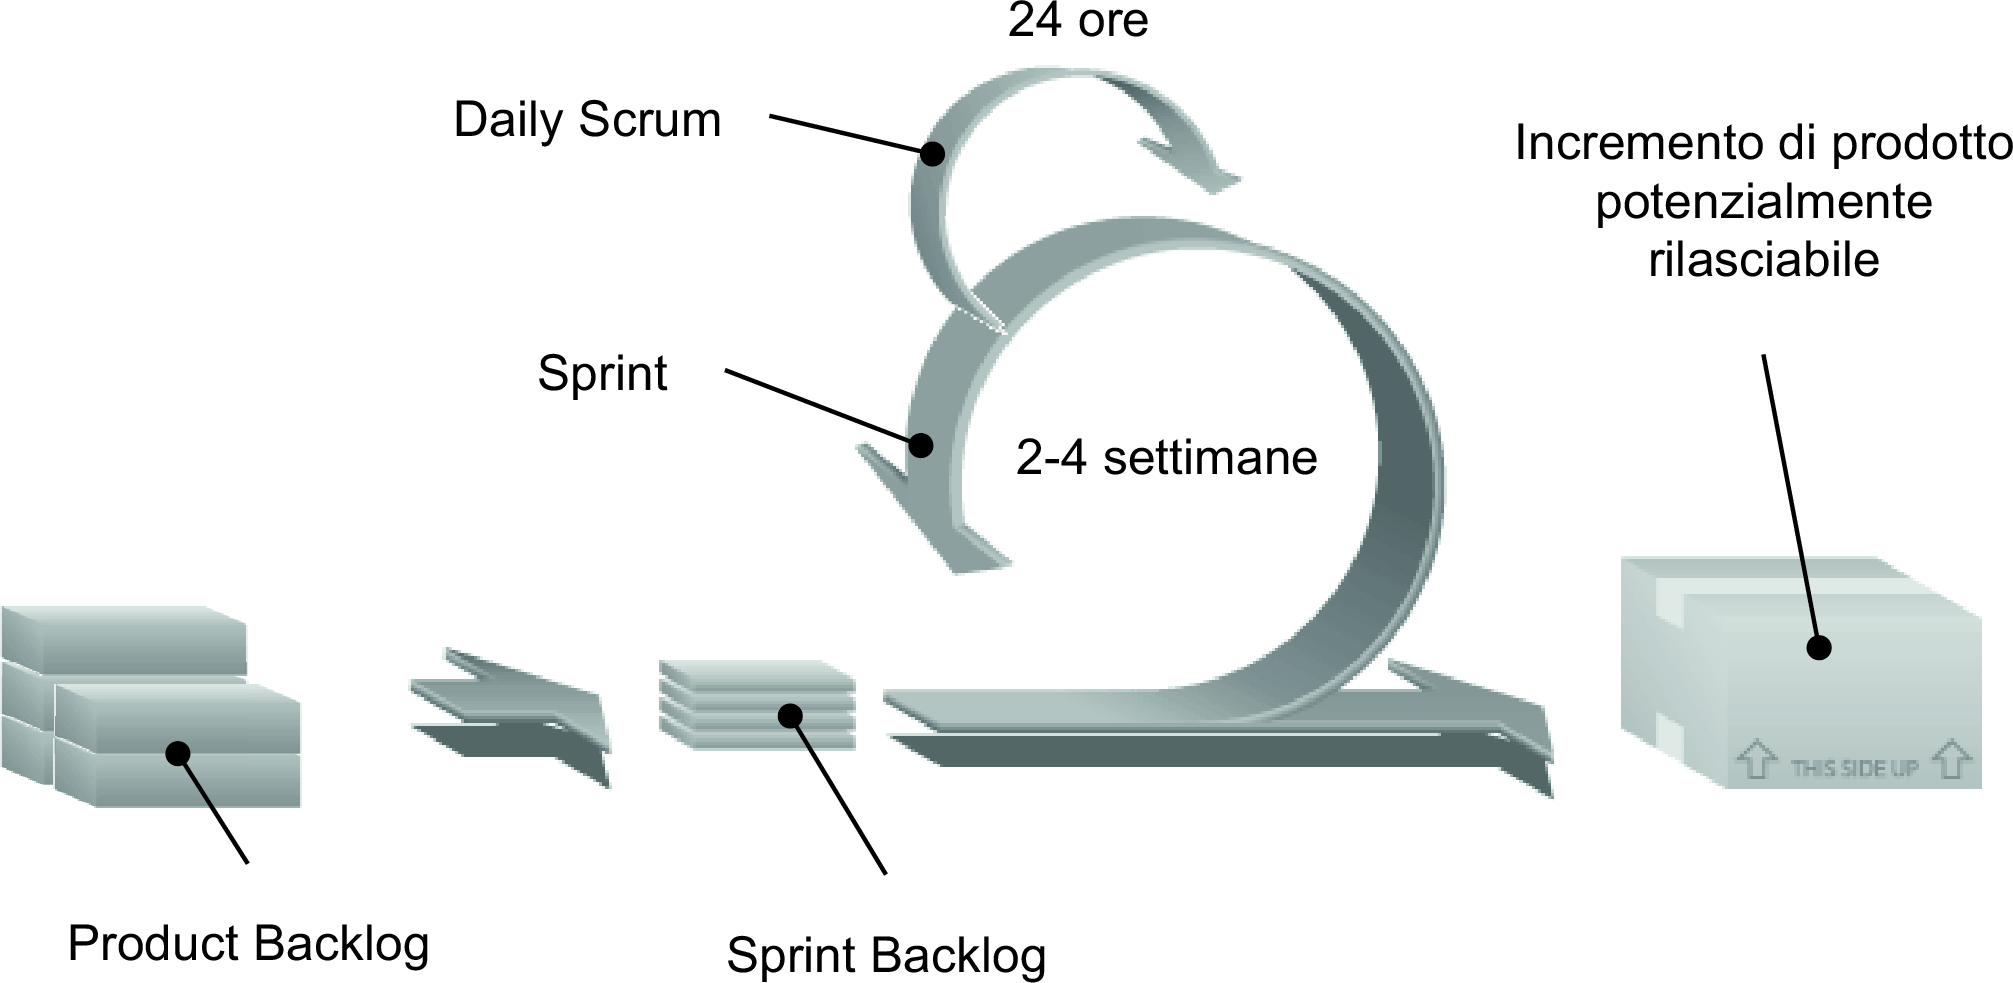
\includegraphics[width = 0.80\textwidth]{Images/23.png}
\end{center}
La caratteristica distintiva di Scrum tra i metodi agili è \textbf{l'enfasi sull'adozione di team auto-organizzanti e auto-organizzati}.
Inoltre, Scrum è basato su un insieme di \textbf{elaborati ed eventi che hanno lo scopo di rendere visibili gli obbiettivi e il progresso delle iterazioni e di favorire un adattamento evolutivo del processo di sviluppo}.
Facciamo un riassunto di alcune delle terminologie viste:
\begin{center}
    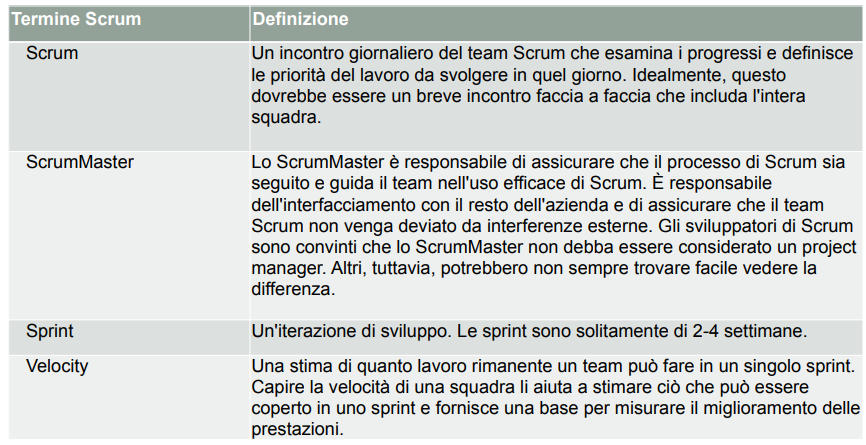
\includegraphics[width = 1\textwidth]{Images/24.png}
\end{center}
\begin{center}
    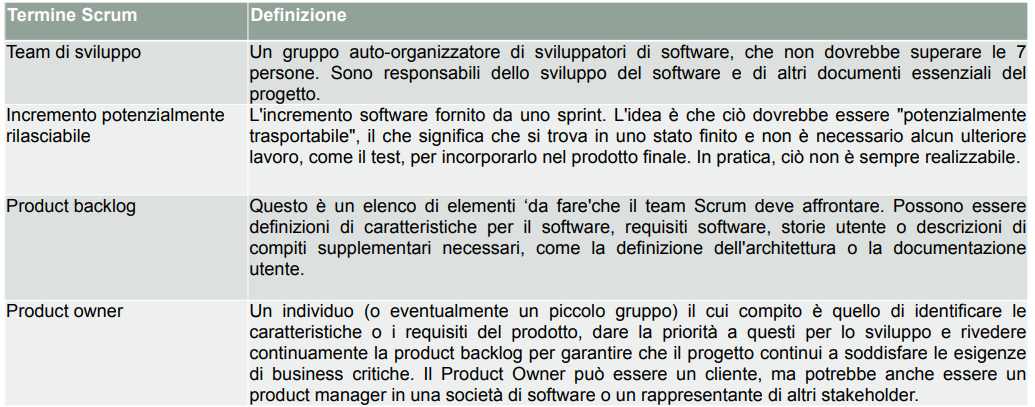
\includegraphics[width = 1.10\textwidth]{Images/25.png}
\end{center}
\section{Iterazione 0: Analisi dei requisiti}
L'iterazione 0 per gli \textbf{studi di caso} enfatizza i concetti fondamentali dell'\textbf{analisi dei requisiti}.
Questa capacità costituisce un \textbf{prerequisito fondamentale} per l'analisi e la progettazione ad oggetti che verranno presentate nelle prossime iterazioni.
Nello sviluppo iterativo è utile avere una "\textbf{iterazione 0}" iniziale, che ha lo scopo di \textbf{definire la visione del software da realizzare} e fornire una \textbf{stima approssimativa} dei tempi e dei costi.
Questo passo iniziale corrisponde alla \textbf{fase di ideazione di UP}. Questa iterazione non ha quindi lo scopo di creare un sistema software eseguibile, ma si concentra soprattutto sull'avvio di altre attività ed elaborati, tra cui, appunto, \textbf{l'analisi dei requisiti}.
\subsection{Ideazione}
La maggior parte dei progetti richiede un breve passo iniziale dove si affrontano i seguenti tipi di domande:
\begin{itemize}
    \item Qual'è la \textbf{visione} e qual'è lo \textbf{studio economico} per questo progetto?
    \item Il progetto è \textbf{fattibile}?
    \item \textbf{Comprare} e/o \textbf{costruire}?
    \item Stima \textbf{approssimativa e non affidabile} dei cosi (ordine di grandezza della spesa)
    \item Dovremmo procedere o fermarci?
\end{itemize}
In UP, l'ideazione è appunto il \textbf{breve} passo iniziale che permette di definire la visione del progetto e di ottenere una \textbf{stima}, approssimativa e non affidabile, dei \textbf{costi} e dei \textbf{tempi} di sviluppo.
A tal fine, l'ideazione richiede \textit{un po' di analisi dei requisiti}, come, per esempio, il 10\% dei \textbf{requisiti funzionali} (casi d'uso) nonché l'analisi dei \textbf{requisiti non funzionali più critici}.
È necessario tenere a mente che \textbf{lo scopo di questa fase non è quello di definire tutti i requisiti}, né quello di generare una stima o un piano di progetto affidabili; se si sta facendo questo allora si sta sovrapponendo il \textbf{pensiero a cascata a UP}.
L'idea è quella di \textbf{effettuare un'indagine sufficiente} per formarsi un'\textbf{idea razionale e giustificabile} sull'obbiettivo generale e sulla fattibilità del sistema software e decidere se \textbf{vale la pena di investire in un'indagine più approfondita} (scopo della fase di \textbf{elaborazione}).
La maggior parte dell'analisi dei requisiti \textbf{avviene durante la fase di elaborazione, in parallelo alle prime attività di programmazione di qualità-produzione e di test}.
Per la maggior parte dei progetti, la fase di ideazione dovrebbe essere \textbf{relativamente breve} (es. una settimana).
Quindi:
\begin{itemize}
    \item \textbf{Ideazione in una frase}: immaginarsi la portata del prodotto, la visione e lo studio economico
    \item \textbf{Il problema che risolve in una frase}: Le parti hanno un \textbf{accordo di base sulla visione del progetto}, e vale la pena investire su un'analisi più seria?
\end{itemize}
Lo scopo dell'ideazione è quindi quello di stabilire una visione iniziale comune per gli obbiettivi del progetto, stabilire se questo è fattibile e decidere se vale la pena di effettuare alcune indagini serie nell'elaborazione.
Se è stato \textbf{deciso a priori che il progetto è fattibile} (per esempio perché il team ha già fatto progetti simili), allora la fase di elaborazione può essere anche \textbf{particolarmente breve}. 
Essa può comprendere il \textbf{primo workshop sui requisiti e la pianificazione per la prima iterazione}, per poi passare direttamente all'elaborazione.
\subsubsection{Elaborati iniziati durante l'ideazione}
\begin{center}
    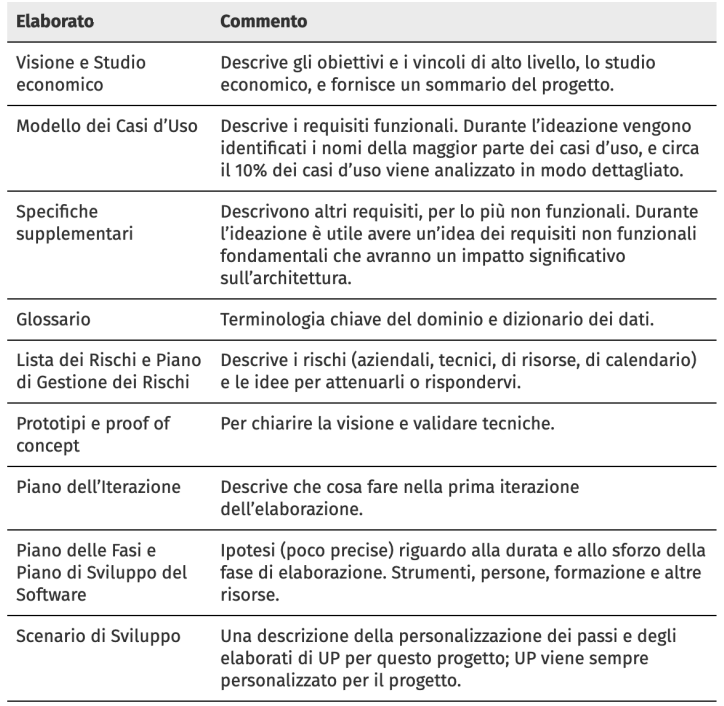
\includegraphics[width = 0.75\textwidth]{Images/26.png}
\end{center}
Ricordiamo che nello sviluppo iterativo, gli elaborati creati in questa fase \textbf{saranno parziali e verranno raffinati durante le prossime iterazione}; inoltre essi \textbf{non devono essere creati se non si ritiene che aggiungano un valore pratico effettivo}.
Si noti che l'ideazione \textbf{può comprendere la programmazione di prototipi} per chiarire alcuni requisiti attraverso (di solito) prototipi \textbf{orientati all'interfaccia utente}.
La tabella sopra mostra un ampio numero di elaborati per questa fase, tuttavia è necessario tenere a mente che \textbf{gli elaborati di UP vanno considerati opzionali} e bisogna scegliere di creare solo quelli necessari.
\subsubsection{Ideazione e UML}
Dato lo scopo dell'ideazione, è probabile che \textbf{non si faccia molto uso di UML in questa fase} se non per i \textbf{semplici diagrammi dei casi d'uso}.
NGli elaborati prodotti in questa fase sono:
ell'ideazione c'è una maggiore enfasi sulla \textbf{comprensione della portata del progetto e del 10\% dei requisiti}; espressi soprattutto in \textbf{forma testuale}.
L'applicazione e la creazione della maggior parte dei diagrammi UML avverrà nella fase di \textbf{elaborazione}.
\subsection{Requisiti evolutivi}
Ogni sistema software ha lo scopo di \textbf{risolvere} un determinato problema di interesse \textbf{per un insieme di utenti}.
A tal fine, il sistema deve di solito fornire un \textbf{insieme di funzionalità}, relative alla \textbf{gestione di certe tipologie di informazioni}.
Inoltre, il sistema deve possedere alcune caratteristiche di \textbf{qualità}, per esempio, in termini di sicurezza, affidabilità, ecc... 
Una possibile definizione di \textbf{requisito} è quindi la seguente:
\begin{Definizione}
    Un \textbf{requisito} è una capacità o una condizione a cui il sistema, e più in generale il progetto, deve essere conforme
\end{Definizione}
I requisiti \textbf{derivano da richieste degli utenti del sistema} (e di altri parti interessate).
Inoltre i requisiti vengono spesso \textbf{formalizzati} in un documento, una specifica o su un altro documento formale.
Ci sono \textbf{due tipi} principali di requisiti:
\begin{itemize}
    \item \textbf{Requisiti funzionali} (comportamentali): Descrivono il comportamento del sistema, in termini di \textbf{funzionalità fornite} ai suoi utenti.
    Questi requisiti sono di solito orientati all'uso del sistema e possono essere espressi, per esempio, sotto forma di \textbf{casi d'uso}.
    I requisiti funzionali comprendono anche gli aspetti \textbf{relativi alle informazioni che il sistema deve gestire}
    \item I \textbf{Requisiti non funzionali} (tutti gli altri requisiti): Non riguardano le specifiche funzioni del sistema ma sono relative a \textbf{proprietà del sistema nel suo complesso}
    (es. sicurezza, prestazioni, usabilità) 
\end{itemize} 
Una sfida primaria nell'analisi dei requisiti \textbf{è trovare, comunicare e ricordare} (il che di solito significa scrivere) ciò che è realmente necessario, in una forma che parli \textbf{chiaramente} al cliente e ai membri del team di sviluppo.
Più generale, UP promuove un insieme di \textbf{best practices}, una delle quali è \textit{gestire i requisiti}; cioè, nel contesto dei desiderata delle parti interessate,  che sono \textbf{poco chiari e inevitabilmente cambieranno}, indica un \textbf{approccio sistematico per trovare, documentare, organizzare e tracciare i requisiti che cambiano di un sistema}.
\begin{center}
    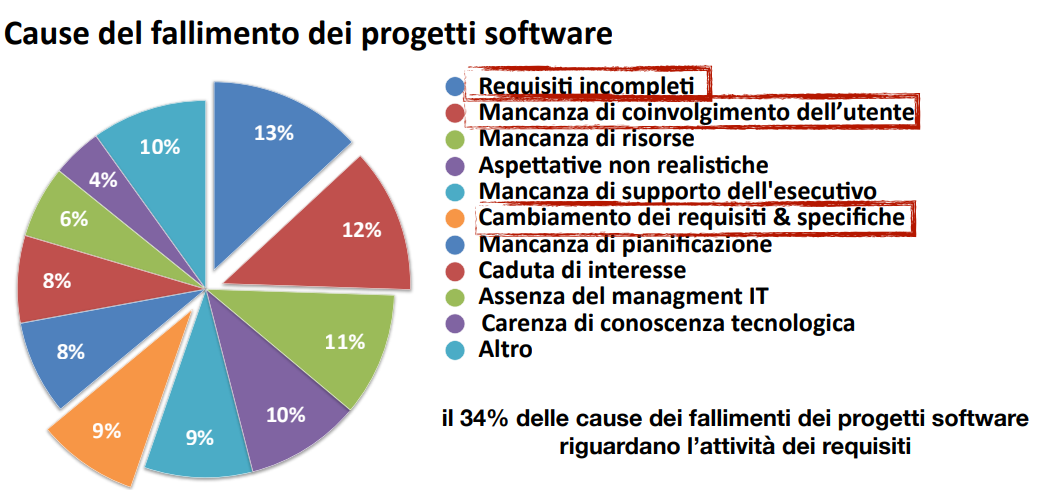
\includegraphics[width = 0.85\textwidth]{Images/27.PNG}
\end{center}
\subsubsection{Proprietà dei requisiti funzionali}
Altri problemi possono insorgere quando vi è \textbf{ambiguità nell'interpretazione dei requisiti funzionali}. Per esempio, la parola \textit{verificare} potrebbe essere interpretata in \textbf{modi diversi} dall'utente e dal programmatore.
In linea di principio, i \textbf{requisiti funzionali} dovrebbero essere:
\begin{itemize}
    \item \textbf{Completi}: Dovrebbero includere la \textbf{definizione di tutti i servizi richiesti}
    \item \textbf{Coerenti}: Non devono \textbf{contenere informazioni contraddittorie}
\end{itemize}
In pratica, tuttavia, molto spesso, a causa della \textbf{complessità del sistema e dell'ambiente}, è impossibile produrre un documento completo e coerente sui requisiti.
\subsubsection{Proprietà dei requisiti non funzionali}
\begin{center}
    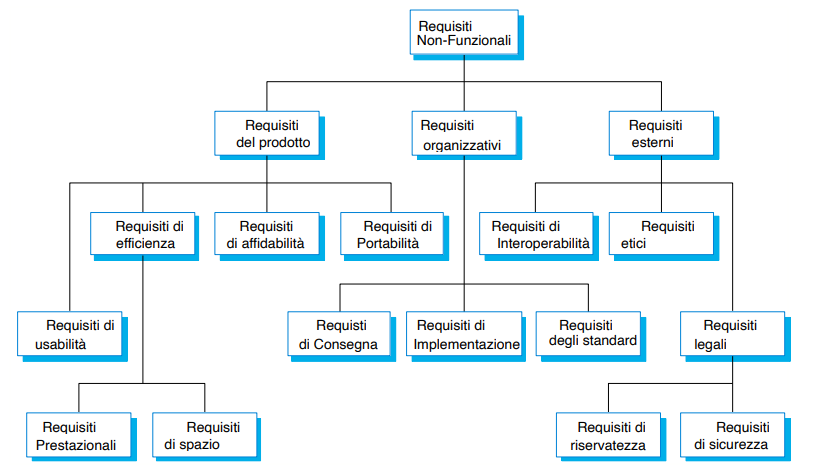
\includegraphics[width = 0.70\textwidth]{Images/28.PNG}
\end{center}
I \textbf{Requisiti non funzionali} definiscono le \textbf{proprietà e i vincoli del sistema}, come ad esempio affidabilità e tempo di risposta; oppure vincoli come la \textbf{capacità dei sistemi di I/O}, le rappresentazioni dei dati nelle interfacce di sistema ecc...
Essi possono \textbf{vincolare il processo di sviluppo} del software in diversi ambiti, come ad esempio quali \textbf{standard di qualità usare} oppure \textbf{quali strumenti di sviluppo usare}.
I requisiti non funzionali potrebbero \textbf{risultare più critici dei requisiti funzionali}. In caso essi non siano soddisfatti, il sistema potrebbe \textbf{risultare inutilizzabile}.
Lo schema sopra rappresenta i \textbf{tipi di requisiti non funzionali}. I requisiti non funzionali possono influire anche sull'architettura \textbf{complessiva} del sistema invece che solo sui singoli componenti.
Un unico requisito non funzionale inoltre può generare \textbf{una serie di requisiti funzionali correlati} che definiscono i \textbf{servizi di sistema necessari} o può generare requisiti che \textbf{limitano quelli già esistenti}.
I requisiti non funzionali possono essere tuttavia \textbf{molto difficili da individuare con precisione} e requisiti imprecisi possono essere \textbf{difficili da verificare}. Quindi, possiamo usare questa distinzione:
\begin{itemize}
    \item \textbf{Obbiettivo}: Un'\textbf{intenzione generale dell'utente}, come, per esempio, la facilità d'uso
    \item \textbf{Requisito funzionale verificabile}: Una \textbf{dichiarazione} che utilizza alcune misure \textbf{oggettivamente verificabili}
\end{itemize}
Gli obbiettivi sono utili agli sviluppatori poiché trasmettono le \textbf{intenzioni degli utenti del sistema}.
Le seguenti sono \textbf{metriche per specificare i requisiti non funzionali}:
\begin{center}
    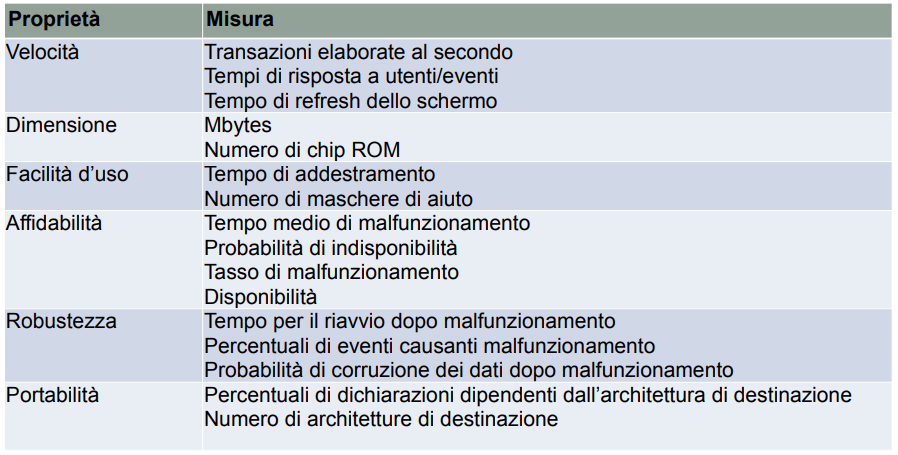
\includegraphics[width = 0.90\textwidth]{Images/29.PNG}
\end{center}
\subsubsection{Requisiti evolutivi e a cascata a confronto}
Un aspetto fondamentale dell'analisi dei requisti è la \textbf{gestione dei requisiti che cambiano}. Una gestione non realistica dei requisiti (e del loro cambiamento) è infatti alla base del \textbf{fallimento di molti progetti software}.
Lo sviluppo iterativo \textbf{abbraccia il cambiamento nei requisiti} come una \textbf{guida} fondamentale per i progetti. Questo aspetto è estremamente importante ed è al centro delle differenze tra \textbf{sviluppo iterativo e sviluppo a cascata}.
In UP e in altri metodi \textbf{evolutivi}, si inizia la programmazione di qualità e il test \textbf{molto prima che tutti i requisiti siano stati definiti} (forse all'inizio della programmazione se ne è definito il 10\%/20\%).
A partire dagli anni ottanta, emersero prove che le convenzioni \textbf{seguite dal modello a cascata} sull'analisi dei requisiti, cioè \textbf{avere un fase di analisi e scrittura dei requisiti} che dovesse descrivere ed individuare \textbf{tutti i requisiti di un sistema}, erano \textbf{basate su principi errati}.
In particolare, la vecchia convenzione considerava il processo di sviluppo del software come un \textbf{tradizionale processo di produzione di massa prevedibile}, dove i requisiti di un prodotto \textbf{hanno un tasso di cambiamento basso}.
Tuttavia, il software rientra nel dominio dello sviluppo di \textbf{nuovi prodotti} con \textbf{tassi di cambiamento alti e con grado di novità e scoperta elevati}. Infatti, in media, nei progetti software il \textbf{25\% dei requisiti cambia}.
Pertanto, qualsiasi metodo che cerchi di \textbf{congelare i requisiti di un sistema} o che si opponga al loro inevitabile cambiamento è \textbf{fondamentalmente difettoso e basato su un falso presupposto}.
Secondo lo studio [Thomas01], effettuato su oltre mille progetti software, il fattore di fallimento più comune è stato il \textbf{tentare di applicare pratiche a cascata}: è stato menzionato come problema principale nell'82\% dei progetti.
\begin{center}
    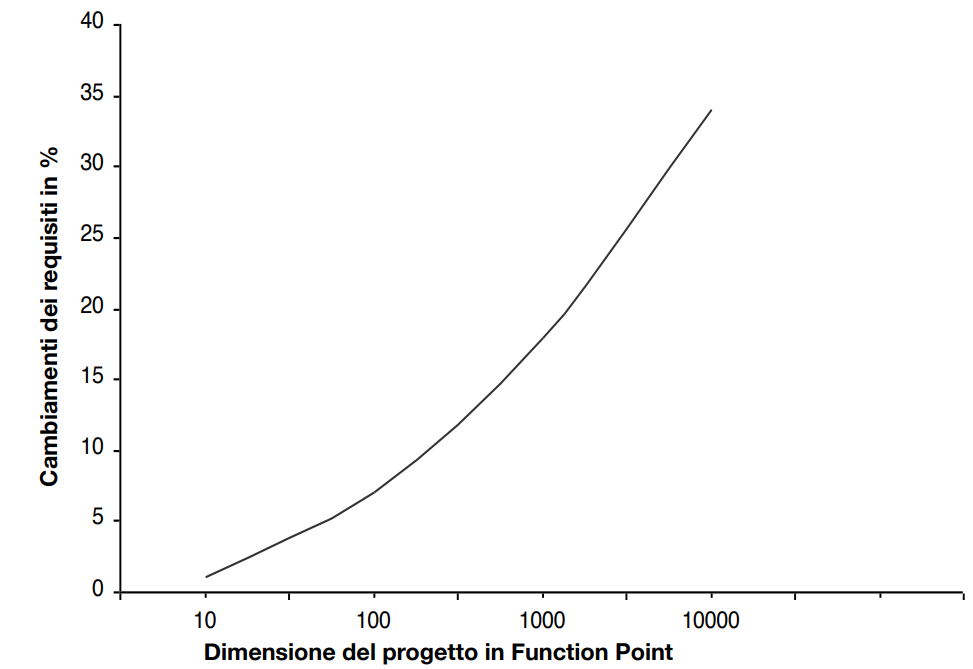
\includegraphics[width = 0.70\textwidth]{Images/15.png}
\end{center}
Un altro importante studio ([Johnson02]), svolto su migliaia di progetti, risponde alla seguente domanda: \textit{se si segue un'analisi dei requisiti a cascata; quante delle caratteristiche specificate inizialmente sono effettivamente utili nel prodotto software finale}?
I risultati sono abbastanza sorprendenti:
\begin{center}
    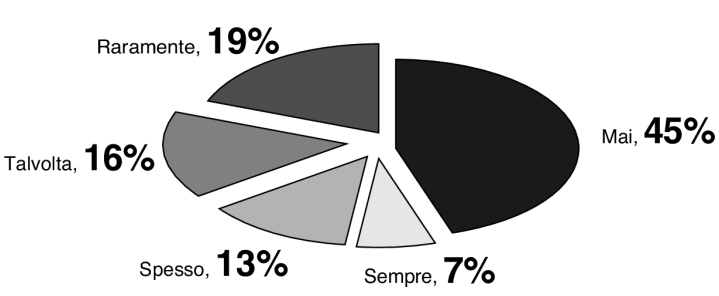
\includegraphics[width = 0.70\textwidth]{Images/30.PNG}
\end{center}
Dunque, quasi il \textbf{65\%} delle caratteristiche specificate secondo un approccio a cascata si è rilevato inutile o poco utile.
Questi risultati non implicano che \textbf{il modo giusto di procedere sia quello di scrivere codice sin dal primo giorno, dimenticandosi dell'analisi dei requisiti}.
Invece, essi indicano che esiste una \textbf{via intermedia}: \textbf{l'analisi dei requisiti iterativa ed evolutiva} combinata con uno sviluppo \textbf{anticipato, iterativo e timeboxed}, nonché \textbf{partecipazione, valutazioni e feedback dei risultati parziali frequenti} da parte delle parti interessate.
\subsubsection{Modi validi per trovare i requisiti}
UP incoraggia un'acquisizione dei requisiti abile, attraverso, diverse tecniche:
\begin{itemize}
    \item \textbf{Scrivere i casi d'uso con gli utenti}
    \item \textbf{Workshop dei requisiti} dove partecipano programmatori e clienti
    \item \textbf{Gruppi di lavoro} con rappresentanti dei clienti
    \item \textbf{Dimostrazione del risultato di ogni iterazione}, per ottenere un feedback istantaneo dal cliente
\end{itemize}
UP accoglie \textbf{qualsiasi metodo di acquisizione dei requisiti} fino a quando esso può aggiungere valore e \textbf{aumentare la partecipazione degli utenti}.
Anche il metodo delle "storie" di XP può essere integrato in UP, tuttavia è una pratica molto difficile da realizzare poiché richiede \textbf{la presenza a tempo pieno del cliente o di un esperto}.
\subsection{Tipi e categorie di requisiti}
Nella gestione dei requisiti è spesso utile utilizzare un qualche sistema di classificazione come \textbf{checklist} per la copertura dei requisiti e per ridurre il rischio di non star tralasciando un qualche importante aspetto del sistema.
Ci sono \textbf{diversi sistemi di qualificazione dei requisiti} ed essi sono pubblicati da \textbf{enti che si occupando di standard}, come ISO, SEI (Software Engineering Institute) ecc... \newline
Ecco alcune categorie principali di requisiti:
\begin{itemize}
    \item \textbf{Funzionale}: Requisito \textbf{funzionale}, caratteristiche e capacità funzionali
    \item \textbf{Usabilità}: Riguarda aspetti legati alla facilità d'uso del sistema; documentazione e aiuto per l'utente
    \item \textbf{Affidabilità}: Riguarda caratteristiche come la \textbf{disponibilità} (la quantità di tempo in cui il sistema è attivo e offre i suoi servizi agli utenti), la capacità del sistema di \textbf{tollerare i guasti} (fault tolerance) o di \textbf{poter essere ripristinato in seguito a fallimenti}
    \item \textbf{Prestazioni}: Riguarda caratteristiche come \textbf{tempi di risposta, throughput, capacità e uso delle risorse}
    \item \textbf{Sicurezza}: Riguarda la capacità del sistema di resistere ad \textbf{usi non autorizzati}, ma al tempo stesso di poter essere utilizzato dai suoi utenti legittimi
    \item \textbf{Sostenibilità}: È l'abilità del sistema software di essere \textbf{facilmente modificabile per consentire miglioramenti e riparazioni}. Riguarda aspetti come \textbf{adattabilità, manutenibilità, verificabilità, localizzazione, configurabilità, compatibilità}
\end{itemize}
Esistono anche altre categorie di requisiti, complementari e secondari, quali per esempio:
\begin{itemize}
    \item \textbf{Vincoli di progetto}: Limitazioni su \textbf{risorse, linguaggi e strumenti da utilizzare, hardware,}... 
    \item \textbf{Interoperabilità}: Vincoli imposti dalla necessità di \textbf{interagire e interfacciarsi con sistemi esterni}.
    \item \textbf{Operazionali}: Gestione del sistema nel suo contesto operativo
    \item \textbf{Fisici}: Per esempio, vincoli sulle dimensioni per l'hardware
    \item \textbf{Legali}: licenze e cose simili
\end{itemize}
Alcuni dei requisiti non funzionali sono chiamati \textbf{attributi di qualità del sistema}.
Fra questi ci sono:
\begin{itemize}
    \item \textbf{Usabilità}
    \item \textbf{Affidabilità}
    \item \textbf{Prestazioni}
    \item \textbf{Sostenibilità}
\end{itemize} 
Gli attributi di qualità hanno una forte influenza sull'architettura del sistema.
\subsection{Requisiti ed elaborati di UP}
UP offre diversi elaborati dei requisiti che, come molti altri elaborati di UP, sono \textbf{opzionali}. I principali sono:
\begin{itemize}
    \item \textbf{Modello dei casi d'uso}: Un insieme di \textbf{scenari tipici dell'utilizzo del sistema}. Usato principalmente per i requisiti funzionali 
    \item \textbf{Specifiche supplementari}: Essenzialmente tutto ciò che \textbf{non rientra nei casi d'uso}. È usato principalmente per i requisiti non funzionali. È anche il posto per registrare delle \textbf{caratteristiche funzionali non espresse o non esprimibili come casi d'uso} (es. la generazione di un report)
    \item \textbf{Glossario}: Nella sua forma più semplice, il glossario definisce i \textbf{termini significativi}. Esso ha anche il ruolo di \textbf{dizionario dei dati} che registra i requisiti relativi ai dati, come \textbf{regole di validazione, valori accettabili} e così via. Il Glossario può definire nel dettaglio \textbf{qualsiasi elemento}, dall'attributo di un oggetto fino al parametro di un'operazione.
    \item \textbf{Visione}: Riassume i \textbf{requisiti ad alto livello} che sono dettagliati nel \textbf{modello dei casi d'uso} e nelle \textbf{specifiche supplementari}; contiene inoltre lo \textbf{studio economico} del progetto. Esso quindi è un \textbf{documento sintetico} usato per apprendere rapidamente le idee principali del progetto.
    \item \textbf{Regole di business}: Le \textbf{regole di business} (o regole di dominio) descrivono di solito requisiti che \textbf{trascendono il dominio del progetto software}. Esse sono richieste nel \textbf{dominio o nel business} ed è possibile che molte applicazioni vi si debbano \textbf{conformare} (es. le leggi fiscali di un certo stato). I dettagli delle regole di dominio \textbf{possono} essere registrati nelle \textbf{specifiche supplementari}, ma poiché di solito sono \textbf{più durature} e \textbf{sono applicabili a più progetti}, inserirle in un elaborato centrale, condiviso tra tutti gli analisti, permette un \textbf{miglior riuso dello sforzo di analisi}. 
\end{itemize}
I requisiti sono scritti come \textbf{frasi in linguaggio naturale} integrate da \textbf{diagrammi e tabelle}.
Il linguaggio naturale è usato perché è \textbf{espressivo, intuitivo e "universale"}, quindi può essere compreso sia dai clienti che dagli utenti.
\subsection{Linee guida per la scrittura dei requisiti}
Possiamo seguire le seguenti linee guida quando scriviamo i requisiti:
\begin{itemize}
    \item Ideare un \textbf{formato standard} ed utilizzarlo per tutti i requisiti
    \item L'utilizzo del linguaggio in modo \textbf{consistente}: utilizzare \textbf{DEVE} per i requisiti obbligatori, \textbf{DOVREBBE} per i requisiti desiderabili
    \item Utilizzare \textbf{l'evidenziazione del testo} per identificare le parti più importanti dei requisiti
    \item \textbf{Evitare il gergo informatico}
    \item Includere una \textbf{spiegazione razionale} del motivo per cui è necessaria una certa disposizione.
\end{itemize}
\subsection{Casi d'uso}
I \textbf{casi d'uso} sono \textbf{storie scritte} di un qualche attore che \textbf{usa un sistema per raggiungere degli obbiettivi}; essi sono ampiamente utilizzati per \textbf{scoprire e registrare i requisiti}.
Essi influenzano molti aspetti di un progetto, compresa \textbf{l'analisi e la progettazione orientata agli oggetti}, tuttavia essi \textbf{NON SONO ELABORATI ORIENTATI AGLI OGGETTI}.
\begin{center}
    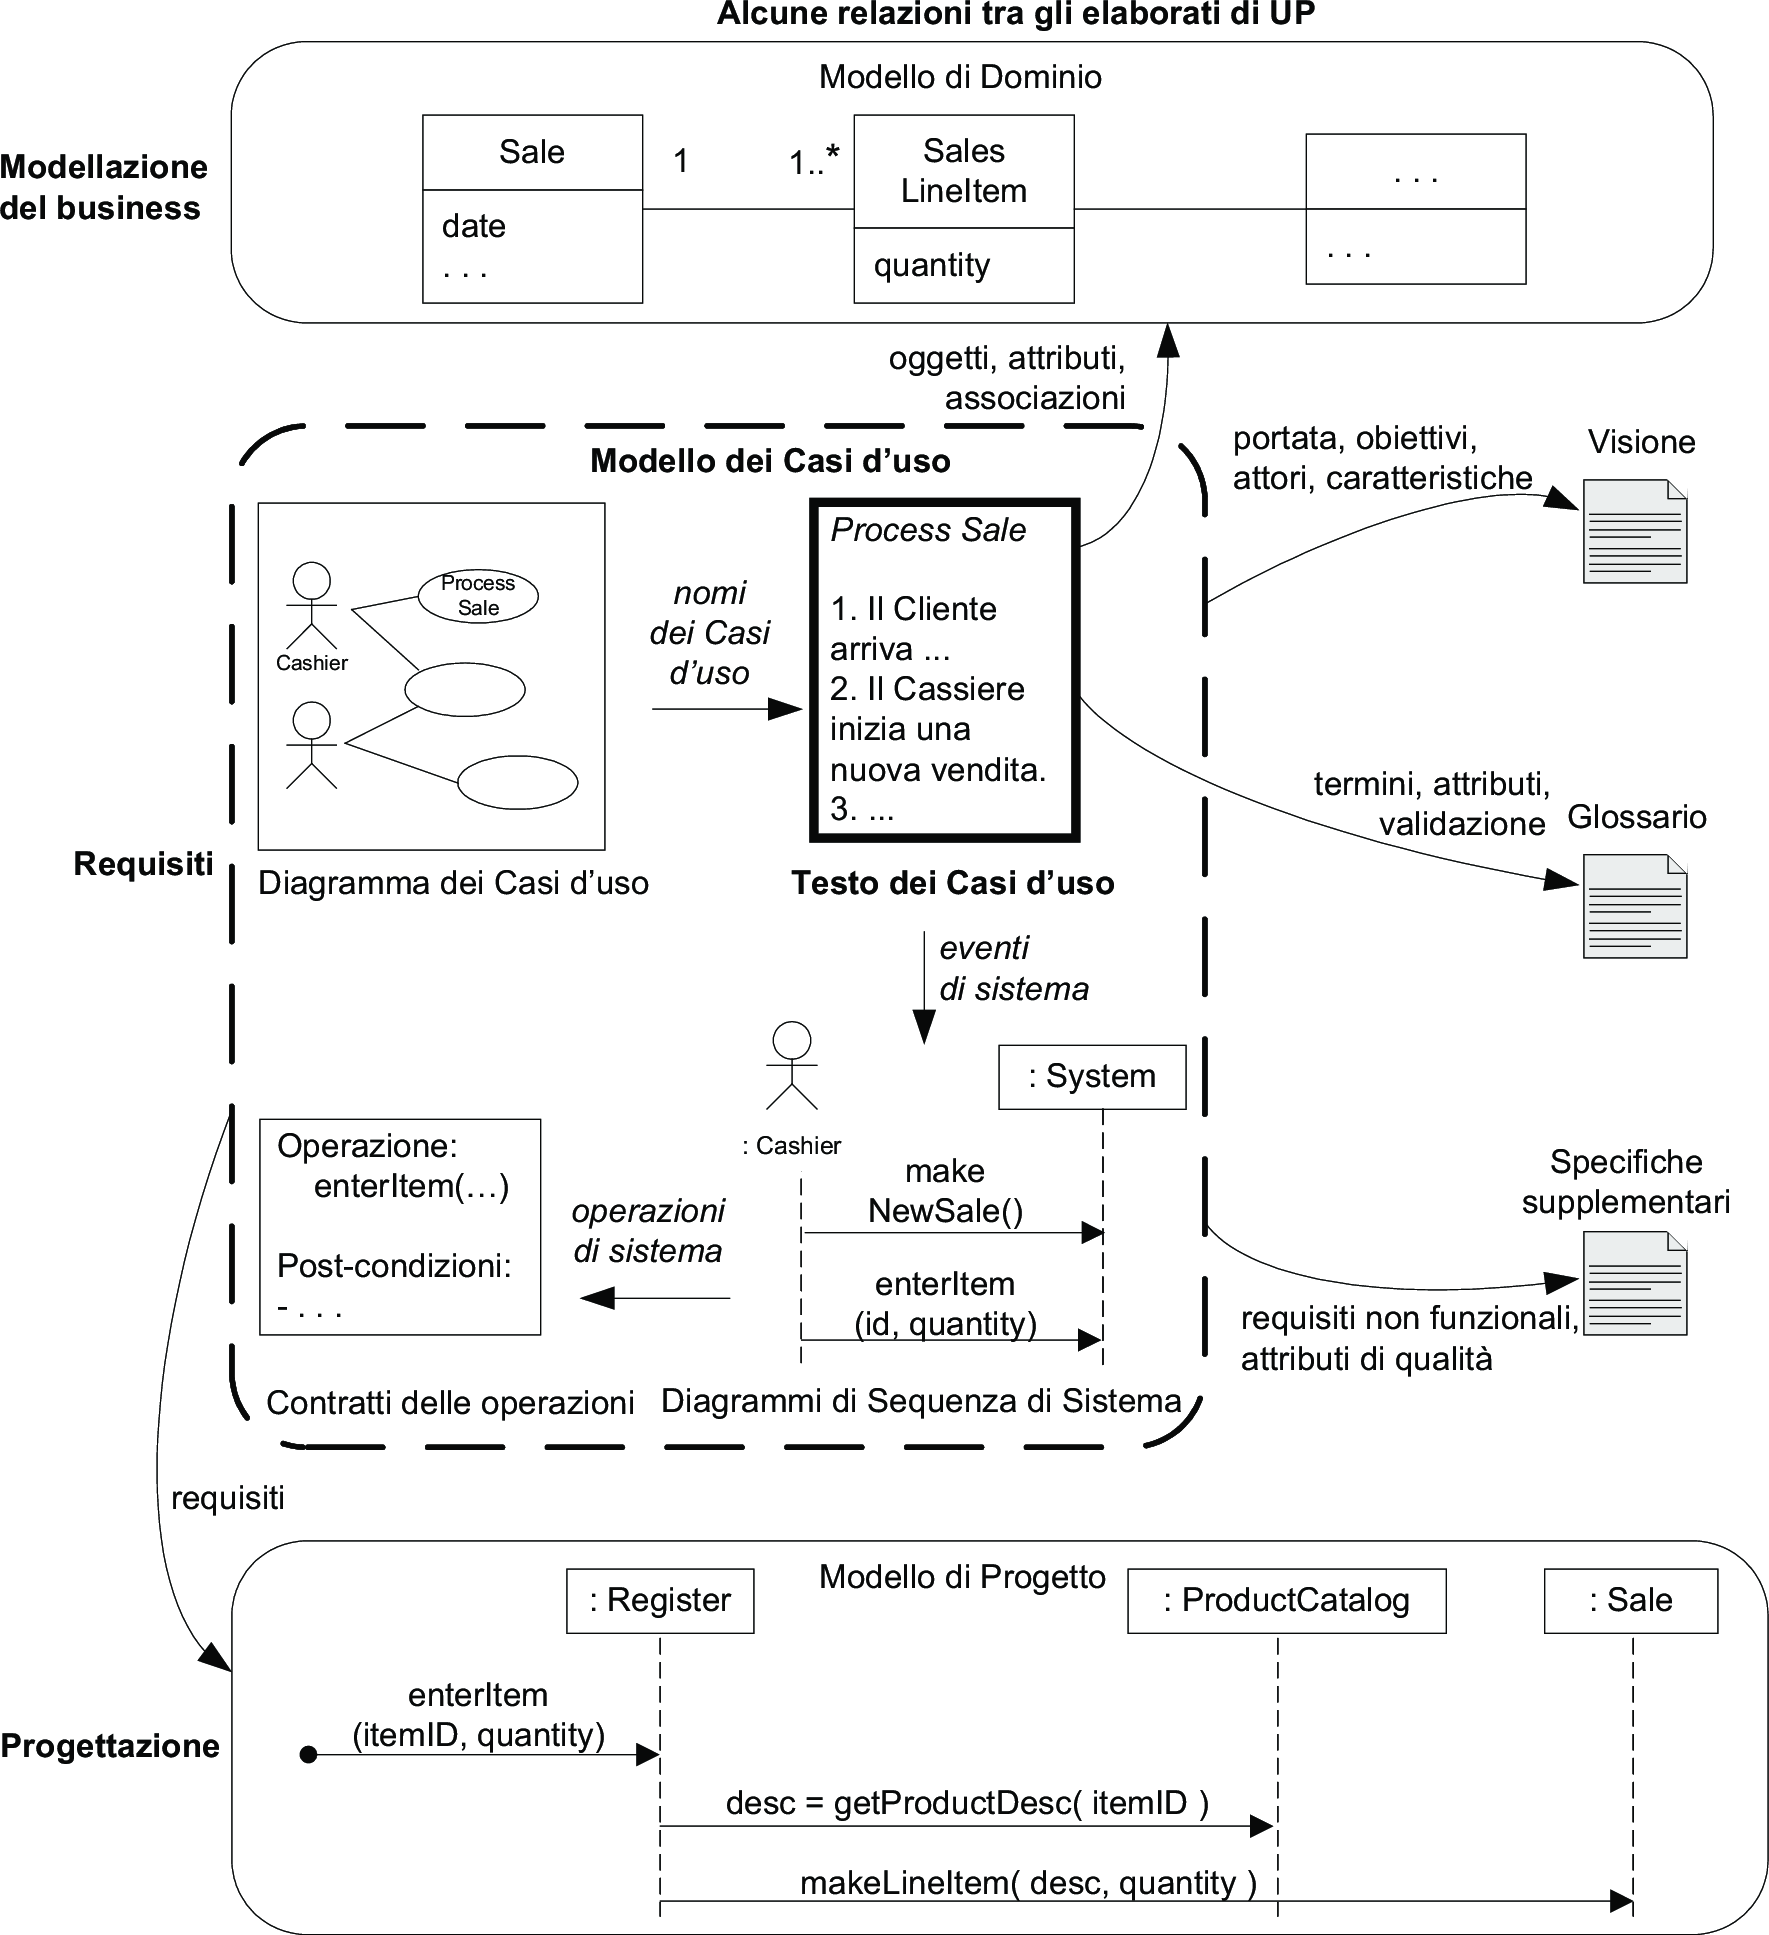
\includegraphics[width = 0.60\textwidth]{Images/31.png}
\end{center}
Innanzitutto, diamo delle definizioni preliminari:
\begin{Definizione}
    Un \textbf{attore} è un qualcosa o un qualcuno dotato di \textbf{comportamento}, come una persona (caratterizzata da un \textbf{ruolo}), un \textbf{sistema informatico} oppure un'\textbf{organizzazione}.
\end{Definizione}
\begin{Definizione}
    Uno \textbf{scenario} (o \textbf{istanza di caso d'uso}) è una \textbf{sequenza specifica di azioni e interazioni tra il sistema e alcuni attori}.
    Uno scenario descrive una \textbf{particolare storia nell'uso del sistema}, ovvero un \textbf{percorso attraverso il caso d'uso}.
\end{Definizione}
\begin{Definizione}
    Un \textbf{caso d'uso} è una \textbf{collezione di scenari correlati}, sia di \textbf{successo} che di \textbf{fallimento}, che descrivono un attore che \textbf{usa un sistema per raggiungere un obbiettivo specifico}.
\end{Definizione}
Oppure
\begin{Definizione}
    Un \textbf{caso d'uso} è un insieme di \textbf{scenari}, in cui ogni scenario è una \textbf{sequenza di azioni} che un sistema esegue per \textbf{produrre un risultato osservabile e di valore per uno specifico attore}
\end{Definizione}
\subsubsection{Modello dei casi d'uso}
UP definisce il \textbf{modello dei casi d'uso} nell'ambito della disciplina dei \textbf{requisiti}.
Si tratta dell'insieme di \textbf{tutti i casi d'uso descritti}; è un modello delle funzionalità del sistema e del suo ambiente.
I casi d'uso \textbf{sono documenti di testo, non diagrammi}, quindi l'attività di scriverli è più un'attività di scrittura di testi, non di disegno di diagrammi.
Il \textbf{modello dei casi d'uso} può includere, opzionalmente, \textbf{un diagramma UML dei casi d'uso} che mostra i nomi dei casi d'uso e degli \textbf{attori} e le \textbf{relazioni} tra essi.
Esso costituisce un buon \textbf{diagramma di contesto} di un sistema e del suo ambiente, oltre a fornire un indice di facile consultazione dei nomi dei casi d'uso.
Seppur i casi d'uso non sono \textbf{orientati agli oggetti}; ciò non costituisce un problema ma anzi, ne ampli \textbf{l'applicabilità e l'utilità}, poiché permettono di rappresentare i \textbf{requisiti come input utile per l'OOA/D classica}
\subsubsection{Perché i casi d'uso}
Molti metodi di analisi sono \textbf{troppo complessi} e vengono compresi sono dagli analisti, ma mettono in confusione l'uomo d'affari medio.
Il mancato coinvolgimento dell'utente è tra le prime ragioni di \textbf{fallimento} dei progetti software [Larman03], e quindi è decisamente opportuno utilizzare tutto ciò che può contribuire al loro coinvolgimento.
I casi d'uso sono un buon \textbf{metodo per mantenere la semplicità e consentire agli esperti di dominio di scrivere essi stessi i casi d'uso} o almeno di \textbf{partecipare alla loro scrittura}.
Un altro valore dei casi d'uso è che mettono in risalto \textbf{gli obbiettivi degli utenti e il loro punto di vista}; i casi d'uso costituiscono la risposta alle domande:
\begin{itemize}
    \item \textbf{Chi} utilizza il sistema?
    \item \textbf{Quali sono} i loro scenari di uso tipici?
    \item \textbf{Quali sono} i loro obbiettivi?
\end{itemize}
Questo pone un'enfasi \textbf{sull'utente}, invece di chiedere semplicemente quali devono essere le \textbf{caratteristiche funzionali del sistema}.
Un'ulteriore punto di forza dei casi d'uso è dato dalla possibilità di \textbf{aumentare o diminuire il loro livello di dettaglio e formalità}.
\subsubsection{I casi d'uso sono requisiti funzionali}
I casi d'uso \textbf{sono} requisiti, soprattutto \textbf{requisiti funzionali o comportamentali}, che indicano cosa il sistema deve fare.
Oltre agli aspetti funzionali, i casi d'uso possono essere \textbf{utilizzati anche per altri tipi di requisiti}, soprattutto se essi sono fortemente correlati ad altri casi d'uso.
In molti metodi moderni, come UP, la scrittura dei casi d'uso è il \textbf{metodo consigliato} per la scoperta e definizione dei \textbf{requisiti}.
Un punto di vista correlato è quello che definisce un caso d'uso come un \textbf{contratto relativo al comportamento di un sistema} [Cockburn01]
\subsubsection{Tipi di attori}
Un attore è \textbf{qualcosa o qualcuno dotato di comportamento}. Anche il \textbf{sistema in discussione} (SuD: System under Discussion) stesso è considerato un attore, quando \textbf{ricorre ad altri sistemi esterni}.
Ci sono diversi tipi di attori:
\begin{itemize}
    \item \textbf{Attori primari}: Utilizza \textbf{direttamente} i servizi del SuD, affinché vengano raggiunti degli obbiettivi utente. È utile identificare gli attori primari per \textbf{trovare gli obbiettivi degli utenti}, poiché essi guidano l'identificazione dei casi d'uso.
    \item \textbf{Attore finale}: Vuole che il SuD sia utilizzato \textbf{affinché si raggiungano i suoi obbiettivi}. Spesso, attore primario e finale \textbf{coincidono}, perché l'attore primario vuole raggiungere i propri obbiettivi usando il SuD. Tuttavia, vi può essere il caso in cui l'attore primario è \textbf{un intermediario che usa il sistema} invece che l'attore finale. È utile identificare gli attori finali per \textbf{trovare gli obbiettivi di questi attori}; che possono essere utili per guidare l'identificazione di altri importanti casi d'uso
    \item \textbf{Attore di supporto}: \textbf{Offre un servizio} (per esempio, informazioni) al SuD. Spesso è un sistema informatico, ma potrebbe essere una persona o un'organizzazione. È utile identificare gli attori di supporto per \textbf{chiarire le interfacce dei sistemi esterni usati dal SuD e i loro protocolli}.
    \item \textbf{Attore fuori scena}: Ha interesse nel \textbf{comportamento del caso d'uso}, ma non è un attore primario, finale o di supporto. È utile identificarli per garantire che \textbf{vengano individuati e soddisfatti tutti gli interessi necessari di tutte le parti interessate}. Gli interessi degli attori fuori scena sono spesso \textbf{sottili e facili da dimenticare} a meno che non vengano \textbf{nominati esplicitamente}.
\end{itemize}
\newpage
\subsubsection{Formati comuni per i casi d'uso}
I casi d'uso possono essere scritti \textbf{usando diversi formati e livelli di formalità}:
\begin{itemize}
    \item \textbf{Formato breve}: Riepilogo conciso di un solo paragrafo, normalmente relativo al solo scenario principale di successo.
    \begin{itemize}
        \item \textbf{Quando va usato?} Durante \textbf{l'analisi iniziale dei requisiti}, per capire rapidamente l'argomento e la portata
    \end{itemize}
    \item \textbf{Formato informale}: Più paragrafi, scritti in maneire \textbf{informale}, relativi a \textbf{vari scenari}
    \begin{itemize}
        \item \textbf{Quando va usato?} Come nel caso del formato breve, solo con un livello di dettaglio maggiore
    \end{itemize}
    \item \textbf{Formato dettagliato}: \textbf{Tutti i passi e tutte le variazioni} sono scritti nel dettaglio; ci sono anche delle \textbf{sezioni di supporto}, come le \textbf{pre-condizioni, le post-condizioni e le garanzie di successo}.
    \begin{itemize}
        \item \textbf{Quando va usato?} Dopo che \textbf{molti casi d'uso sono stati definiti e scritti in formato breve}, alcuni casi d'uso (circa il 10\%) che hanno maggiore valore e che sono \textbf{più significativi dal punto di vista dell'architettura} vengono scritti in formato dettagliato. Nelle iterazioni successive, anche gli altri casi d'uso verranno via via scritti in formato dettagliato.
    \end{itemize}
\end{itemize}
Un buon template (e quello più diffuso dagli anni 90) è stato definito da \textbf{Alistair Cockburn}:
\begin{center}
    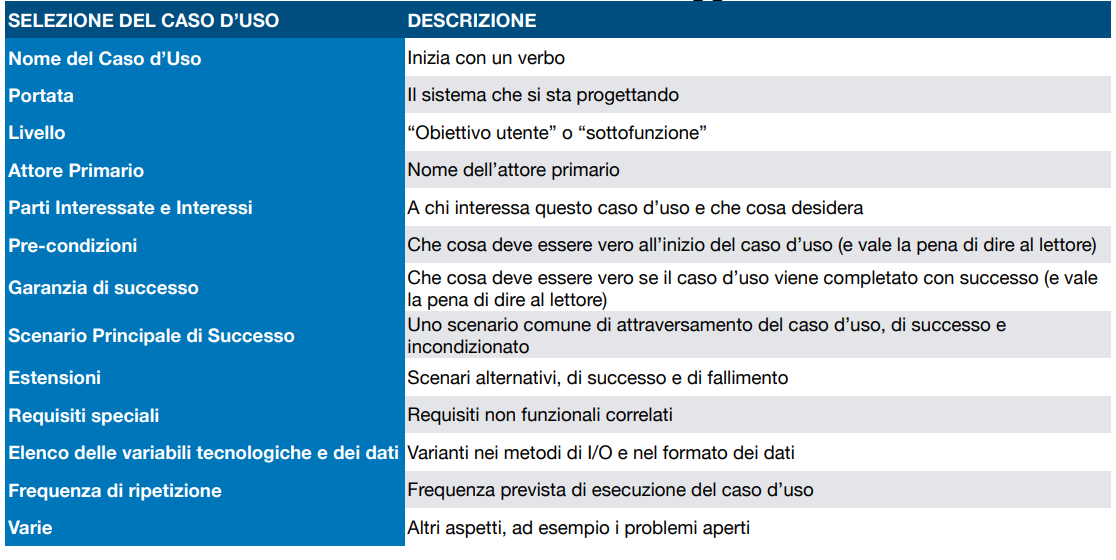
\includegraphics[width = 1.05\textwidth]{Images/32.PNG}
\end{center}
Vediamo come interpretare le sue varie sezioni:
\begin{itemize}
    \item \textbf{Elementi del preambolo}: Il preambolo è composto da tutto ciò che precede lo \textbf{scenario principale e le estensioni}. Contiene informazioni che è importante leggere prima degli scenari del caso d'uso
    \begin{itemize}
        \item \textbf{Portata}: La portata descrive i \textbf{confini del sistema} in via di progettazione. Normalmente un caso d'uso descrive l'utilizzo di un sistema software. In questo caso viene chiamato \textbf{caso d'uso di sistema}.
        Adottando una portata più ampia, i casi d'uso possono anche descrivere il \textbf{modo in cui un'azienda o un'organizzazione viene utilizzata dai suoi clienti o dai suoi soci}. Una simile descrizione prende il nome di\textbf{caso d'uso di business}.
        \item \textbf{Livello}: I casi d'uso vengono classificati con un \textbf{livello}; possibili livelli, tra gli altri, sono il \textbf{livello obbiettivo utente} e il \textbf{livello di sottofunzione}.
        \begin{itemize}
            \item \textbf{Obbiettivo utente}: un caso d'uso a livello di obbiettivo utente è il tipo più comune di caso d'uso; esso descrive gli \textbf{scenari con cui un attore primario può portare a termine il suo lavoro, raggiungendo i suoi obbiettivi}.
            Ciò corrisponde approssimativamente a un \textbf{processo di business elementare} (EBP) nell'ingegneria dei processi di business.
            \item \textbf{Sottofunzione}: Un caso d'uso a livello di sottofunzione descrive invece dei \textbf{sotto-passi}, richiesti come \textbf{supporto al raggiungimento di un obbiettivo utente}.
        \end{itemize}
        \item \textbf{Attore finale e attore primario}: L'attore \textbf{finale} è l'attore che vuole raggiungere un obbiettivo, e questo richiede l'esecuzione dei servizi del sistema.
        L'attore \textbf{primario} è l'attore che \textbf{usa direttamente il sistema}. Di solito i due coincidono, ma è possibile che l'attore finale sia un \textbf{intermediario}.
        \item \textbf{Elenco delle parti interessate degli interessi}: Le parti interessate e i loro interessi \textbf{suggeriscono e limitano ciò che il sistema deve fare}. Per dirlo con le parole di Cockburn:
        \textit{Il sistema definisce un contratto tra le parti interessate, dove i casi d'uso descrivono nel dettaglio gli aspetti comportamentali di questo contratto... \newline Il caso d'uso come contratto per il comportamento raccoglie tutti e soli i comportamenti relativi alla soddisfazione degli interessi delle parti interessate}.
        Questo consente di rispondere alla domanda: "\textbf{Che cosa va scritto nel caso d'uso?}"; la risposta è: "\textbf{Ciò che serve a soddisfare tutti gli interessi delle parti interessate}".
        Inoltre, iniziando a scrivere un caso d'uso partendo dai relativi interessi delle parti interessate, si ha a disposizione un metodo per ricordare quali dovrebbero essere le \textbf{responsabilità dettagliate del sistema}.
    \end{itemize}
    \item \textbf{Pre-condizioni e garanzie di successo (post-condizioni)}: Le \textbf{pre-condizioni} descrivono \textbf{cosa deve essere sempre vero all'inizio del caso d'uso}.
    Le pre-condizioni \textbf{non vengono verificate all'interno del caso d'uso} ma si presuppongono vere. Normalmente una pre-condizione implica che \textbf{lo scenario di un'altro caso d'uso sia stato completato con successo}.
    È necessario notare che vale la pena di scrivere \textbf{solamente le pre-condizioni non banali o che vale la pena descrivere al lettore}.
    Le \textbf{garanzie di successo} o \textbf{post-condizioni} affermano \textbf{cosa deve essere vero quando è stato completato con successo il caso d'uso}, ovvero quando si completa \textbf{lo scenario principale di successo} o un percoso alternativo.
    La garanzia \textbf{deve soddisfare tutte le esigenze delle parti interessate}. Anche in questo caso, vale la pena di scrivere \textbf{solo le post-condizioni non ovvie o significative}.
    \item \textbf{Scenario principale di successo e i suoi passi (Flusso di base)}: Lo scenario principale di successo viene anche chiamato \textbf{happy path} oppure \textbf{flusso di base} o \textbf{flusso tipico}.
    Esso descrive \textbf{un percorso di successo comune} che soddisfa gli interessi di tutte le parti interessate. Lo scenario principale è costituito da una \textbf{sequenza di passi numerati}, che può contenere \textbf{passi da ripetere più volte}, ma che di solito non comprende alcuna condizione o diramazione (rimandate alla sezione delle estensioni).
    I passi che formano lo scenario possono essere di tre tipi:
    \begin{enumerate}
        \item \textbf{Un'interazione tra attori}. Anche il sistema deve essere considerato un attore. I casi più comuni sono:
        \begin{enumerate}
            \item \textbf{Un attore} (utente) \textbf{interagisce con il sistema}, inserendo dati o effettuando una richiesta
            \item \textbf{Il sistema interagisce con un attore} (utente), comunicandogli dei dati o fornendogli una risposta
            \item \textbf{Il sistema interagisce con altri sistemi}
        \end{enumerate}
        \item Un \textbf{cambiamento di stato} da parte del sistema
        \item \textbf{Una validazione}
    \end{enumerate}  
    Il primo di un caso d'uso \textbf{non rientra sempre in questa classificazione}, ma talvolta può indicare \textbf{l'evento trigger} che scatena l'esecuzione dello scenario.
    Similmente, nemmeno l'ultimo passo rientra sempre in questa classificazione, ma può descrivere il fatto che \textbf{l'attore ha effettivamente conseguito i suoi obbiettivi}.
    I nomi degli attori di solito vengono scritti \textbf{con l'iniziale maiuscola} per distinguerli meglio.
    Per indicare una ripetizione di passi, si \textbf{indica testualmente che i passi da n a k vanno ripetuti}
    \item \textbf{Estensioni (o Flussi alternativi)}: In genere,un caso d'uso è composto da molti scenari. Lo scenario principale di successo è solo uno di qeusti scenari.
    Le \textbf{estensioni} hanno lo scopo di descrivere tutti gli altri scenari, sia di \textbf{successo} che di \textbf{fallimento}.
    Per questo, le estensioni comprendono solitamente la \textbf{maggior parte del testo di un caso d'uso}.
    Per descrivere tutti i possibili scenari, è preferibile scriverli \textbf{sotto forma di diramazioni dello scenario principale di successo}. Ciò permette di scrivere un caso d'uso in modo compatto.
    Inoltre, questo modo di procedere è \textbf{compatibile} con le successive attività di analisi, progettazione e implementazione.
    Nella scrittura completa dei casi d'uso, la combinazione del flusso di base e degli altri scenari descritti dalle estensioni \textbf{dovrebbe soddisfare quasi tutti gli interessi delle parte interessate}.
    Tuttavia, alcuni interessi potrebbero essere \textbf{requisiti non funzionali} e quindi essere descritti nelle \textbf{Specifiche supplementari} invece che nei casi d'uso.
    Un'estensione è composta da due parti: \textbf{la condizione} e la \textbf{gestione}; quindi nel seguente modo:
    \begin{center}
        \textit{<numero\_passo/i><lettera\_identificativa>.<Condizione>}
    \end{center}
    Quando è possibile, la condizione deve essere scritta come \textbf{qualcosa che possa essere rilevato dal sistema o da un attore}.
    La sintassi per una diramazione è la seguente:
    \begin{itemize}
        \item Se si vuole descrivere una \textbf{diramazione che parte da un singolo passo}, si usa la sintassi descritta sopra
        \item Se si vuole descrivere una \textbf{diramazione la cui gestione comprende una serie di passi}, si usa la sintassi:
        \begin{center}
            \textit{<passo\_inizio-passo\_fine><lettera\_identificativa>.<Condizione>}
        \end{center}
        Ciò indica anche che il flusso alternativo può essere gestito nell'ambito della sequenza di passi \textbf{"passo\_inizio e passo\_fine"}.
        \item In alcuni casi, i punti di estensione sono \textbf{abbastanza complessi}. Questo può essere un motivo per \textbf{esprimere l'estensione come un caso d'uso separato} con ulteriori estensioni.
        È quindi possibile avere \textbf{estensioni annidate in altre estensioni}.
        \item Se si desidera descrivere una \textbf{condizione di estensione relativa a tutti o molti passi}, si possono utilizzare le etichette \textit{*a, *b, ...}
        \item Talvolta un caso d'uso si dirama \textbf{per eseguire un'altro caso d'uso}. L'esecuzione di un'altro caso d'uso è di solito indicata da una \underline{sottolineatura} del nome del caso d'uso eseguito.
        L'esecuzione di un altro caso d'uso \textbf{deve essere esplicitata come un punto del flusso dell'estensione}.
    \end{itemize}
    Per concludere, le estensioni possono essere usate per \textbf{gestire almeno tre tipi di situazioni principali}:\
    \begin{enumerate}
        \item L'attore vuole che l'esecuzione del caso d'uso \textbf{proceda in modo diverso da quanto previsto dallo scenario principale}.
        \item Il caso d'uso \textbf{procede diversamente da quanto previsto nello scenario principale} ed è il \textbf{sistema che se ne accorge} mentre esegue un'azione o una validazione.
        \item Un passo nello scenario principale \textbf{descrive un'azione generica o astratta}, mentre le estensioni relative a questo passo \textbf{descrivono le possibili azioni specifiche o concrete per eseguire il passo}.
    \end{enumerate}
    \item \textbf{Requisti speciali}: Se un requisito non funzionale, un'attributo di qualità o un vincolo \textbf{si riferiscono in modo specifico a un caso d'uso}, allora è bene scriverlo \textbf{insieme al caso d'uso}. Potrebbe trattarsi di qualità come prestazioni, affidabilità ecc... 
    Registrare questi requisiti insieme al caso d'uso è il consiglio classico di UP, soprattutto se il caso d'uso \textbf{viene scritto prima}. Tuttavia, molti professionisti trovano utile \textbf{spostare e riunire tutti i requisiti funzionali nelle Specifiche supplementari};
    questo favorisce la gestione dei contenuti, la comprensione e la leggibilità, anche perché questi requisiti vanno di solito considerati come un \textbf{tutt'uno} durante \textbf{l'analisi architetturale}.
    \item \textbf{Elenco delle varianti tecnologiche e dei dati}: Spesso ci sono variazioni tecnologiche nel \textbf{modo in cui qualcosa deve essere fatto}, ma non nella sostanza delle cose;
    è importante \textbf{registrare tali varianti} nel caso d'uso. Le \textbf{varianti tecnologiche} possono essere quindi \textbf{vincoli tecnici, imposti da una parte interessata, relativo alle tecnologie da utilizzare}. Si noti che questo è un vincolo precoce della progettazione e che quindi, in generale, sarebbe meglio \textbf{evitare di imporre};
    tuttavia a volte \textbf{è inevitabile oppure ovvio doverlo fare}.
    È inoltre necessario capire \textbf{le varianti nel formato dei dati}; cioè in quali modi le informazioni del sistema possono essere rappresentati.
\end{itemize}
\subsubsection{Linea guida: scrivere in uno stile essenziale}
L'analista di sistema deve essere in grado di \textbf{distinguere il modo in cui si raggiunge uno scopo e lo scopo in sé}. Esaminando la gerarchia degli obbiettivi ("Qual è l'obbiettivo di quell'obbiettivo"), l'analista deve \textbf{giungere a degli obbiettivi indipendenti dai meccanismi}.
Questo processo di scoperta dell'\textbf{obbiettivo radice}, di livello più alto, può suggerire soluzioni \textbf{migliori e nuove}.
Tuttavia, per rispondere adeguatamente alla domanda "Dovrei utilizzare una certa tecnologia?" è necessario anche fare un'\textbf{analisi dell'usabilità di essa} nel contesto in cui ci si trova.
Questa idea è stata riassunta da Cockburn con la frase "\textit{ignorare l'interfaccia utente, concentrarsi sullo scopo}". La sua motivazione è stata analizzata più a fondo da \textbf{Larry Costantine}, il quale giudica \textbf{essenziale} lo stile di \textbf{scrittura} quando esso evita i \textbf{dettagli della UI} e si concentra sullo \textbf{scopo reale dell'utente}.
In uno stile di scrittura essenziale, la narrativa di un caso d'uso viene espressa a livello delle \textbf{intenzioni dell'utente} e delle \textbf{responsabilità} del sistema, anziché con riferimenti ad azioni concrete.
Queste intenzioni e responsabilità rimangono \textbf{indipendenti dai dettagli tecnologici e dai movimenti degli attori} soprattutto quelli relativi all'UI.
\begin{center}
    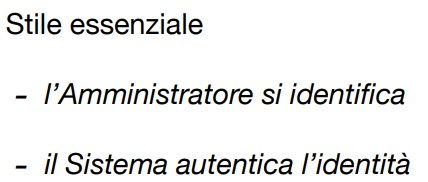
\includegraphics[width = 0.35\textwidth]{Images/33.png}
\end{center}
In alternativa, esiste uno \textbf{concreto} per la scrittura dei casi d'uso. In questo stile, le decisioni sull'interfaccia utente sono \textbf{incorporate nel testo} del caso d'uso.
Il testo può anche mostrare delle schermate, discutere la navigazione delle finestre, la manipolazione degli elementi della GUI ecc... 
I casi d'uso concreti possono costruire un aiuto valido nella \textbf{progettazione di GUI concrete} o dettagliate, in una fase successiva, ma \textbf{non sono adatti durante le attività iniziali dell'analisi dei requisiti}; come lo è invece lo stile \textbf{essenziale}.
\begin{center}
    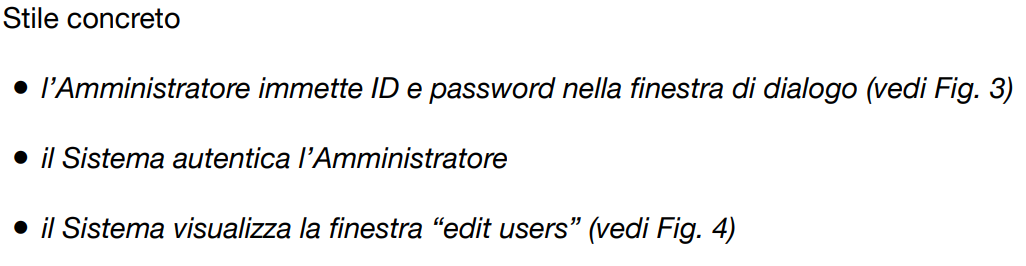
\includegraphics[width = 0.65\textwidth]{Images/34.png}
\end{center}
\subsubsection{Linea guida: scrivere casi d'uso concisi}
Per facilitare la lettura dei requisiti, è perciò opportuno scrivere i casi d'uso in \textbf{modo conciso e allo stesso tempo completo} (con una chiara indicazione di soggetto e verbo e di eventuali frasi subordinate).
\subsubsection{Linea guida: scrivere casi d'uso a scatola nera}
I \textbf{casi d'uso a scatola nera} sono il tipo più comune e consigliato; non descrivono il funzionamento interno del sistema, i suoi componenti o aspetti relativi al suo progetto.
Piuttosto, il sistema è descritto come \textbf{dotato di responsabilità}. Questa è una metafora comune e unificante nel pensare orientato agli oggetti;
gli elementi software \textbf{hanno responsabilità} e collaborano con altri elementi \textbf{dotati di responsabilità}.
Usando i casi d'uso a scatola nera per \textbf{definire la responsabilità del sistema} è possibile specificare che \textbf{cosa} deve fare il sistema senza specificare il \textbf{come}.
Durante l'analisi dei requisiti bisogna specificare il \textbf{comportamento esterno del sistema}, considerato a scatola nera, evitando di prendere decisione sul \textbf{come il sistema effettua le sue operazioni}.
Successivamente, durante la progettazione, andrà creata una \textbf{soluzione che soddisfa le specifiche}.
\begin{center}
    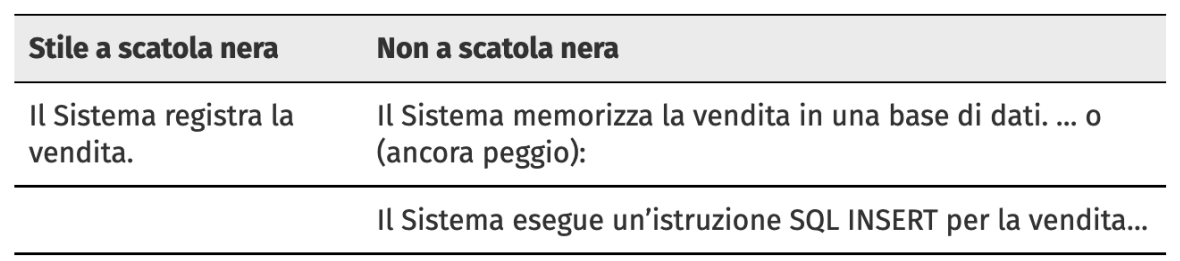
\includegraphics[width = 1\textwidth]{Images/35.png}
\end{center}
\subsubsection{Linea guida: adottare un punto di vista dell'attore e dell'attore-obbiettivo}
La seguente definizione di caso d'uso di RUP è stata formulata dall'inventore dei casi d'uso, \textbf{Ivar Jacobson}:
\begin{center}
    \textit{Un caso d'uso è un insieme di istanze di casi d'uso, in cui ciascuna istanza è una sequenza di azioni che un sistema esegue per produrre un risultato osservabile e di valore per uno specifico attore}
\end{center}
La frase "un risultato osservabile e di valore per uno specifico attore" è un concetto sottile ma importante, che Jacobson considera \textbf{cruciale}, poiché pone l'accento su due atteggiamenti da tenere nel corso dell'analisi dei requisiti:
\begin{itemize}
    \item Scrivere requisiti \textbf{concentrandosi sugli utenti o attori di un sistema}, chiedendo quali sono i loro obbiettivi e le situazioni tipiche.
    \item Concentrarsi sulla \textbf{comprensione di ciò che l'attore considera un risultato di valore} 
\end{itemize}
Seppur possa sembrare banale fornire un valore osservabile per l'utente e concentrarsi sugli obbiettivi tipici degli utenti, l'ingegneria del software è piena di progetti falliti che non hanno saputo fornire agi utenti ciò di cui avevano realmente bisogno.
Il vecchio approccio basato sull'elencazione delle caratteristiche e delle funzioni per descrivere i requisiti può influire negativamente sul processo di sviluppo poiché \textbf{non porta a formulare domande a chi deve utilizzare il prodotto}.
\subsubsection{Linea guida: Come trovare i casi d'uso}
I casi d'uso hanno come scopo quello di soddisfare gli obbiettivi degli attori primari. La procedura base per trovarli è la seguente:
\begin{enumerate}
    \item \textbf{Scegliere i confini del sistema}: Di che tipo di sistema stiamo parlando? Per questo studio di caso, il SuD è \textbf{il sistema stesso}.
    Tutto ciò che è al suo esterno \textbf{è fuori dai confini del sistema}. Per chiarire la definizione dei confini del sistema in corso di progettazione, è utile sapere che gli attori primari e gli attori di supporto sono \textbf{considerati esterni al sistema}.
    Una volta individuati gli attori esterni, i confini del sistema \textbf{diventano più chiari}.
    \item \textbf{Identificare gli attori primari}: Coloro che raggiungono i propri obbiettivi attraverso \textbf{l'utilizzo dei servizi del sistema}
    \item \textbf{Identificare gli obbiettivi di ciascun attore primario}
    \begin{itemize}
        \item Non è naturale cercare di identificare, in stretta sequenza, prima gli attori primari e poi i loro obbiettivi.
        In un workshop sui requisiti, le persone effettuano un brainstorming e \textbf{considerano insieme entrambi gli aspetti}.
        Alcune volte sono gli \textbf{obbiettivi a svelare gli attori} o viceversa.
        Oltre agli attori primari e agli obbiettivi più evidenti, le seguenti domande possono aiutare a identificarne altri:
        \begin{itemize}
            \item Chi avvia il sistema?
            \item Chi si occupa della gestione degli utenti e della sicurezza?
            \item Esiste un processo di monitoraggio che riavvia il sistema se si verifica un errore?
            \item Come vengono gestiti gli aggiornamenti software?
            \item Sono aggiornamenti automatici o a richiesta?
            \item Oltre agli attori primari \textit{umani}, ci sono sistemi software o robotizzati esterni che utilizzano i servizi del sistema?
            \item Chi si occupa dell'amministrazione del sistema?
            \item Il "tempo" è un \textit{attore del sistema}? Nel senso che il sistema esegue operazioni in risposta ad alcuni eventi temporali?
            \item Chi valuta le attività e le prestazioni del sistema?
            \item Chi valuta i log? Vi si accede da remoto?
            \item Chi viene avvisato quando si verificano errori o guasti?
        \end{itemize}
        Ci sono almeno due approcci per \textbf{organizzare gli attori e i loro obbiettivi}:
        \begin{enumerate}
            \item Man mano che vengono scoperti, vengono \textbf{disegnati in un diagramma dei casi d'uso}, chiamando i casi d'uso come gli obbiettivi
            \item Scrivere \textbf{dapprima un elenco attori-obbiettivi}, rivederlo e raffinarlo, per poi \textbf{disegnare il diagramma dei casi d'uso}
        \end{enumerate}
        Se si crea un elenco attori-obbiettivi allora, in termini di elaborati UP, è utile riportare una tabella simile nell'elaborato \textbf{Visione}:
        \begin{center}
            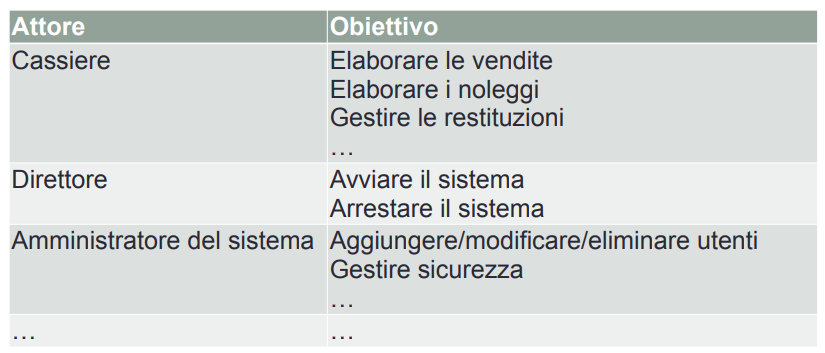
\includegraphics[width = 0.70\textwidth]{Images/36.png}
        \end{center}
        Gli attori hanno \textbf{degli obbiettivi e utilizzano le applicazioni per raggiungerli}.
        La modellazione dei casi d'uso è interessata a \textbf{trovare questi attori e i rispettivi obbiettivi} e creare soluzioni che producono un risultato di valore.
        Questo sposta leggermente l'interesse del \textbf{modellatore del caso d'uso}. Anziché chiedere "\textit{Quali sono le attività svolte?}" si chiederà:
        \begin{center}
            \textit{Chi utilizza il sistema e quali sono i suoi obbiettivi?}
        \end{center}
        È necessario anche identificare \textbf{l'attore primario} del sistema. Ciò non è sempre evidente e dipende \textbf{dai confini del sistema in corso di progettazione}.
        In un caso d'uso di un sistema POS per esempio, potrebbe avere come \textbf{attore primario il cassiere}, poiché è la persona che \textbf{utilizza il sistema per soddisfare i suoi obbiettivi}, tuttavia il cliente \textbf{è considerabile come attore "finale" del caso d'suo} poiché, magari, il caso d'uso soddisfa \textbf{principalmente gli obbiettivi del cliente}.
        \begin{center}
            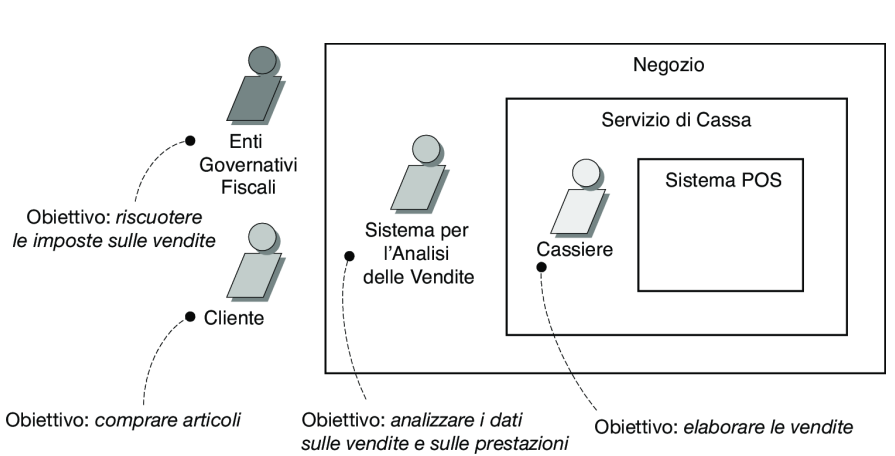
\includegraphics[width = 0.80\textwidth]{Images/37.png}
        \end{center}
        Un'ultimo approccio per trovare gli attori e i loro obbiettivi è \textbf{basato sull'identificazione di eventi esterni al sistema}. 
        Per esempio: \textit{Quali sono? Da dove provengono? Perché?}.
        \begin{center}
            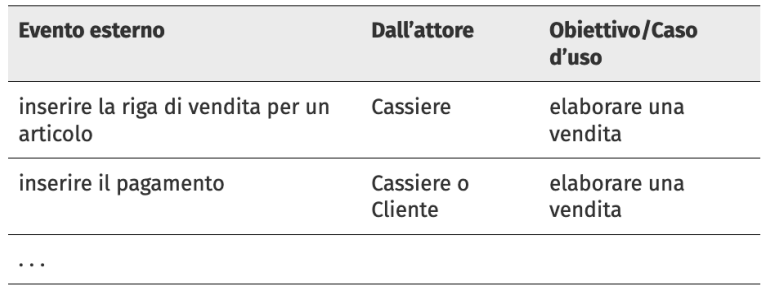
\includegraphics[width = 0.55\textwidth]{Images/38.png}
        \end{center}
    \end{itemize}
     \item \textbf{Definire i casi d'uso che soddisfano gli obbiettivi degli utenti}: il loro nome va scelto \textbf{in base all'obbiettivo}. 
     Di solito, i casi d'uso a livello di \textbf{obbiettivo utente} sono in \textbf{corrispondenza biunivoca} con gli \textbf{obbiettivi degli utenti}; tuttavia c'è più un di un'eccezione a questa regola.
     In generale, va definito definito un \textbf{caso d'uso per ciascuno obbiettivo utente}. È opportuno assegnare al caso d'uso un nome simile all'obbiettivo utente.L
     La linea guida è che \textbf{i nomi dei casi d'uso deve iniziare con un verbo}.
     Un'eccezione comune alla scelta di un caso d'uso per \textbf{obbiettivo} è quella che \textbf{riunisce gli obbiettivi separati CRUD} in un unico \textbf{caso d'uso CRUD}.
     In questo caso, il caso d'uso potrà iniziare con la parola \textit{gestisci} seguita dalla cosa che si vuole gestire.
\end{enumerate}
\subsubsection{Linea guida: Verificare l'utilità dei casi d'uso}
Quali sono i casi d'uso \textbf{validi}? Piuttosto che chiedere questo è più pratico chiedersi \textbf{Qual è un livello utile per esprimere i casi d'uso nell'analisi dei requisiti software}?
Ci sono diverse regole pratiche, tra cui:
\begin{itemize}
    \item \textbf{Test del capo}: Il capo vi chiede: "Cosa avete fatto tutto il giorno?" e voi rispondete di aver fatto \textbf{tutto il giorno qualcosa}. Il vostro capo sarà facile?
    Se non lo è, il caso d'uso non \textbf{supera il test del capo}, il che significa che non è fortemente \textbf{mirato a ottenere risultati il cui valore sia misurabile}.
    Potrebbe essere un caso d'uso a un \textbf{livello più basso}, ma non al livello a cui è desiderabile concentrarsi durante l'analisi dei requisiti.
    Ciò non significa che \textbf{bisogna sempre ignorare i casi d'uso che non superano il test del capo}; a volte il livello di un caso d'uso è basso, quindi non supera il test del capo, ma può invece risultare \textbf{complesso e importante}
    \item \textbf{Test EBP}: La nozione di \textbf{Processo di Business Elementare} (Elementary Business Process, \textbf{EBP}) deriva dal settore dell'ingegneria dei processi da business: \newline
    \textit{Un processo di business elementare è un'attività svolta da una persona in un determinato tempo e luogo, in risposta ad un evento di business, che aggiunge un valore di business misurabile e lascia dati in uno stato consistente} \newline
    La linea guida in questi casi è quindi quella di \textbf{concentrarsi sui casi d'uso che corrispondono a degli EBP}.
    La definizione di EBP tuttavia non deve essere presa in maniera troppo letterale: un caso d'uso fallisce come EBP se ci sono due persone che effettuano l'operazione?
    Probabilmente no, ma il \textbf{tono della definizione è più o meno corretto}.
    Non è un singolo passo; anzi lo scenario principale di successo sarà formato da \textbf{cinque-dieci passi}.
    Non occorrono giorni e sessioni multiple; è \textbf{un'attività eseguita in una sola sessione di lavoro} e probabilmente richiede un lasso di tempo che va dai pochi minuti all'ora.
    Come nella definizione di UP, \textbf{enfatizza l'aggiunta di un valore di business osservabile o misurabile e giunge a una situazione in cui il sistema e i dati sono in uno stato stabile e consistente}.
    \item \textbf{Test della dimensione}: Un caso d'uso è \textbf{raramente costituito da una singola azione o passo}; normalmente comprende diversi passi e nel suo formato dettagliato richiede spesso dalle 3 alle 10 pagine di testo.
    Un errore comune nella modellazione dei casi d'uso è \textbf{definire un caso d'uso formato da un singolo passo}, all'interno di una sequenza di passi correlati. Si può intravedere l'errore \textbf{delle sue dimensioni ridotte}.
\end{itemize}
Benché la maggior parte dei casi d'uso dovrebbe soddisfare i test proposti; ci sono delle eccezioni comuni.
Talvolta è utile scrivere casi d'uso \textbf{separati a livello di sottofunzione} che rappresentano attività secondarie o passi all'interno di un normale caso d'uso a livello EBP.
Per esempio, un'attività secondaria o un'estensione di un certo caso d'uso \textbf{potrebbe essere ripetuta in più casi d'uso di base}.
In questo caso è preferibile \textbf{separarla in un proprio caso d'uso}, anche se non soddisfa pienamente il test EBP.
Un caso d'uso potrebbe non superare il \textbf{test del capo}, ma essere sufficientemente complesso da \textbf{richiedere un'analisi accurata}.
\subsubsection{Definizione: livello dei casi d'uso}
I casi d'uso possono essere scritti a diversi \textbf{livelli}, con riferimento all'obbiettivo che rappresentano:
\begin{itemize}
    \item \textbf{Livello di obbiettivo utente}: Nell'analisi dei requisiti per un sistema software è utile concentrarsi principalmente sui casi d'uso EBP.
    Un caso d'uso di questo tipo è detto \textbf{a livello di obbiettivo utente}, poiché consente all'utente di \textbf{raggiungere l'obbiettivo tramite un solo utilizzo del sistema}
    \item \textbf{Livello di sotto-funzione}: Un caso d'uso a \textbf{livello di sotto-funzione} indica invece un \textbf{passo complesso che il sistema deve compiere nell'ambito di un'altro caso d'uso}.
    La modellazione di questo tipo di casi d'uso è utile quando è necessario indicare a fattor comune delle \textbf{sequenze di passi condivisi da più casi d'uso}.
    \item \textbf{Livello di sommario}: Un caso d'uso \textbf{a livello di sommario} indica un caso d'uso la cui esecuzione ha un lasso temporale d'esecuzione \textbf{mediamente più lungo degli altri casi d'uso} (ore, giorni, mesi, anni ecc...)
    Questi casi d'uso sono utili per \textbf{descrivere una visione complessiva sugli obbiettivi del sistema}. Tuttavia, essi non forniscono direttamente dei requisiti da sviluppare per il sistema software.
    Un caso d'uso di questo tipo \textbf{contiene più casi d'uso a livello obbiettivo utente}
\end{itemize}
\subsection{Diagramma UML dei casi d'uso}
UML fornisce una notazione dei \textbf{diagrammi dei casi d'uso} che consente di utilizzare i nomi e gli attori dei casi d'uso nonché le relazioni tra essi.
Si ricorda tuttavia che l'attività di descrizione dei casi d'uso riguarda \textbf{scrivere testo, non disegnare diagrammi}.
Basta quindi modellare solo un \textbf{semplice diagramma dei casi d'uso insieme ad un elenco attori-obbiettivi}.
Tuttavia, un diagramma dei casi d'uso rappresenta un \textbf{ottimo quadro del contesto di un sistema} poiché esso costituisce un buon \textbf{diagramma di contesto}, che consente di mostrare i confini del sistema.
È quindi un utile strumento di comunicazione che \textbf{riassume il comportamento del sistema e i suoi attori}.
\begin{center}
    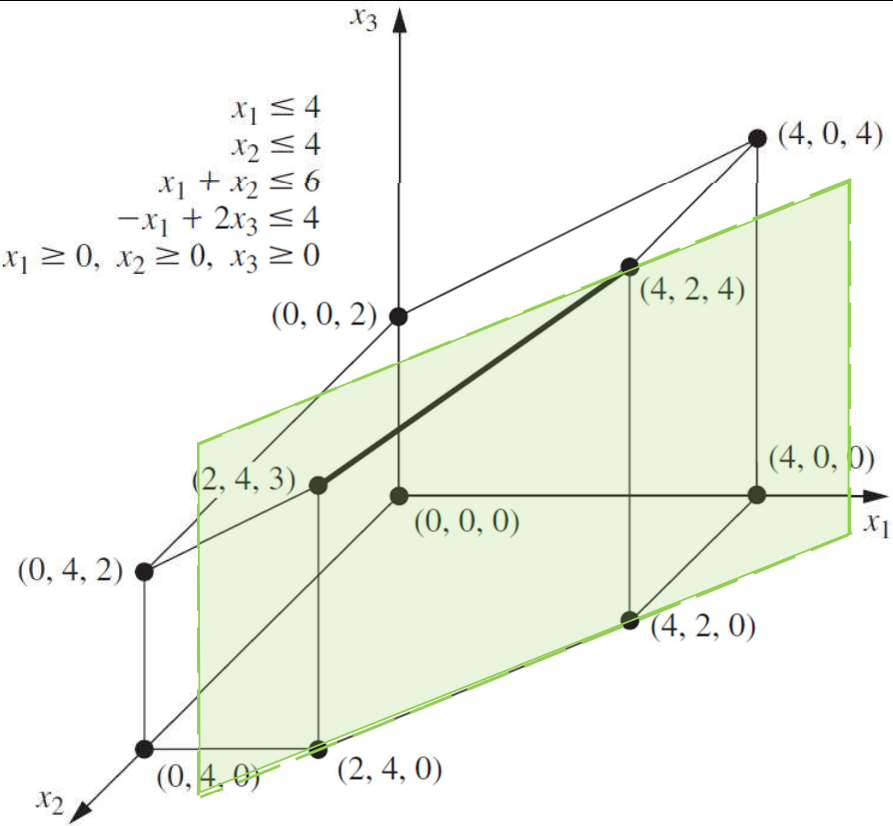
\includegraphics[width = 0.85\textwidth]{Images/39.png}
\end{center}
Si noti il rettangolo nella figura sopra con scritto "actor" tra virgolette basse.
Questa sintassi \textbf{indica parole chiave o stereotipi UML}. Per motivi di chiarezza, alcuni preferiscono modellare gli attori che sono \textbf{enti informatici esterni usando la notazione a rettangolo}
\begin{center}
    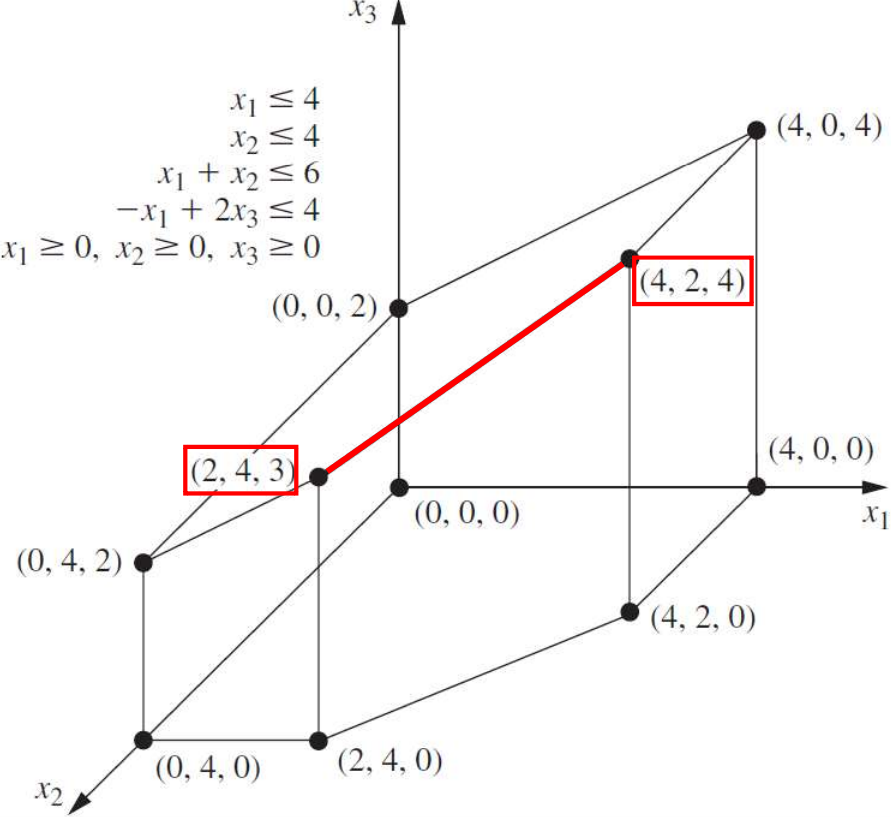
\includegraphics[width = 0.75\textwidth]{Images/40.png}
\end{center}
\subsubsection{Relazione di associazione attore-caso d'uso}
Un'\textbf{associazione} tra un attore e un caso d'uso è un \textbf{canale di comunicazione} tra i due.
Essa è rappresentata con una \textbf{linea continua} e può essere \textbf{sia orientata che non orientata}.
In particolare:
\begin{itemize}
    \item \textbf{Direzione}: chi da inizio all'interazione
    \item \textbf{Nessuna direzione}: entrambe le parti possono dare inizio all'interazione
\end{itemize}
\begin{center}
    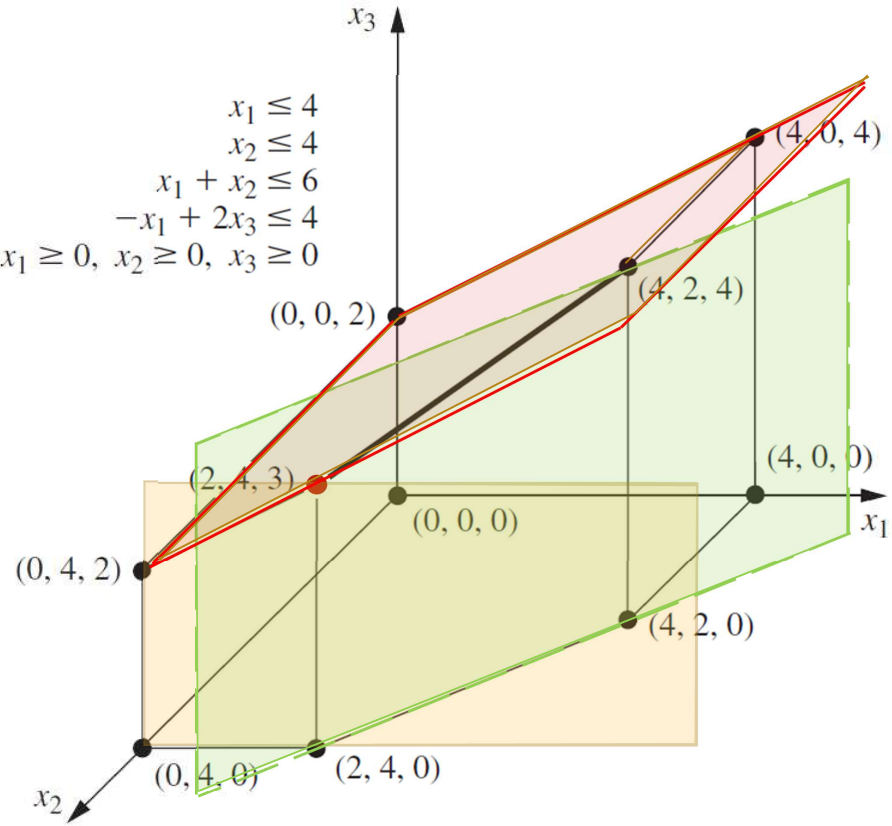
\includegraphics[width = 0.20\textwidth]{Images/41.png}
\end{center}
\subsubsection{Relazione di inclusione}
La \textbf{relazione di inclusione} è la relazione tra casi d'uso \textbf{più frequente e importante}.
È comune avere \textbf{comportamenti parziali in comune tra diversi casi d'uso}; quindi anziché duplicare il testo del caso d'uso, è opportuno separarlo in un proprio caso d'uso \textbf{a livello di sotto-funzione} e indicare la sua inclusione.
Quando viene realizzata una relazione di inclusione, \textbf{il caso d'uso incluso viene eseguito completamente quando viene raggiunto il punto di inclusione}
\begin{center}
    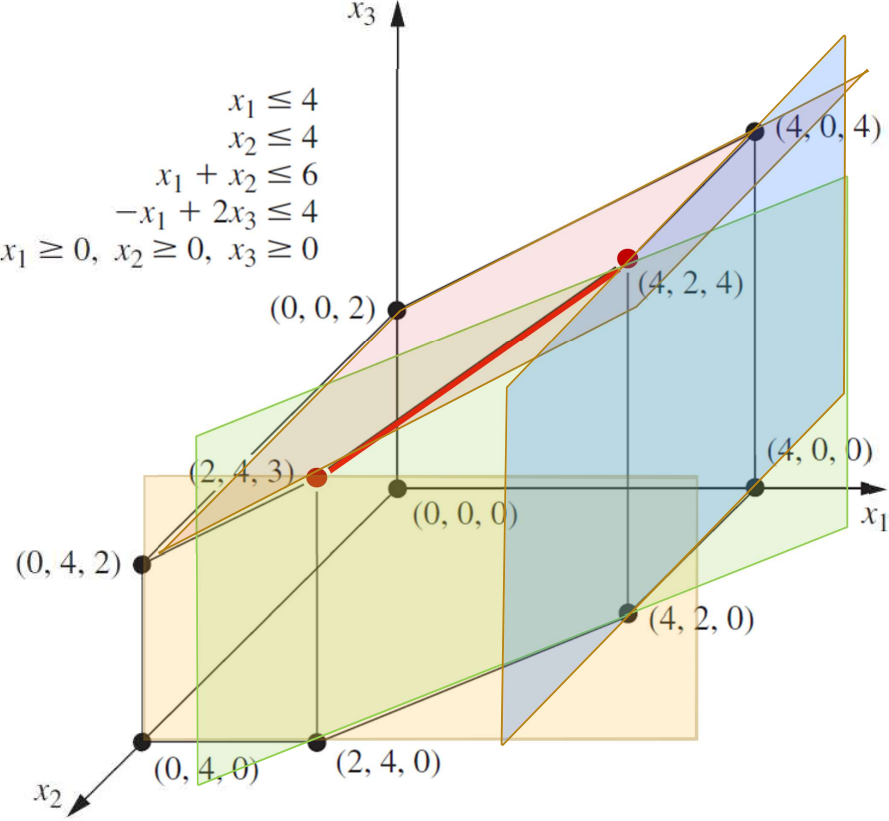
\includegraphics[width = 0.80\textwidth]{Images/42.png}
\end{center}
Nei diagrammi dei casi d'uso, la relazione di include viene espressa nel seguente modo:
\begin{center}
    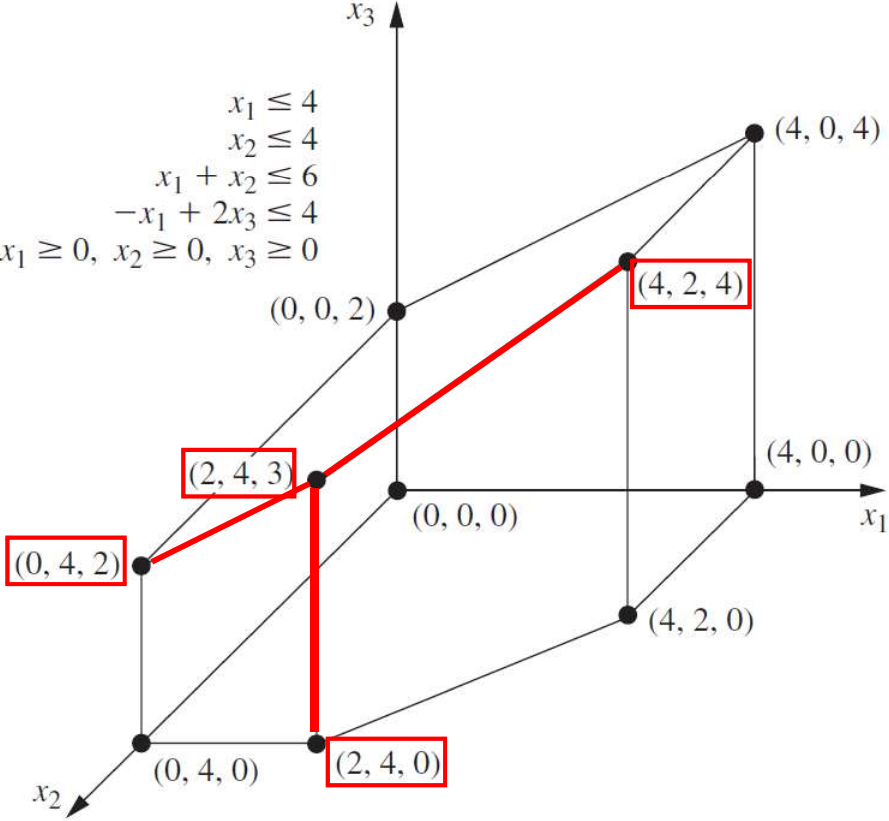
\includegraphics[width = 0.85\textwidth]{Images/43.png}
\end{center}
Nei casi d'uso dettagliati, una notazione semplice e preferibile per indicare la relazione di include \textbf{consiste semplicemente nel sottolineare il caso d'uso incluso} (o evidenziarlo in qualche modo).
Una linea guida semplice e pratica per capire quando usare la relazione di inlcude è offerta da \textbf{Fowler}: \textit{usare la relazione di include quando ci si ripete in due o più casi d'uso separati e si desidera evitare la ripetizione}.
Un'altra motivazione è quella di \textbf{voler scomporre un caso d'uso più complesso per facilitarne la comprensione}.
Un altro uso della relazione di include è per descrivere la \textbf{gestione di un evento asincrono}. La notazione di base per questi casi d'uso è quella di utilizzare la sintassi "\textit{*a, *b, ...}"
Si ricordi che queste possono indicare che l'evento si può \textbf{verificare in qualsiasi momento}. Una notazione minore è quella di indicare \textbf{un'etichetta intervallo} (es. 3-9a) per indicare che l'evento asincrono si può verificare all'interno del flusso di un numero elevato di passi, ma non in tutti.
\begin{center}
    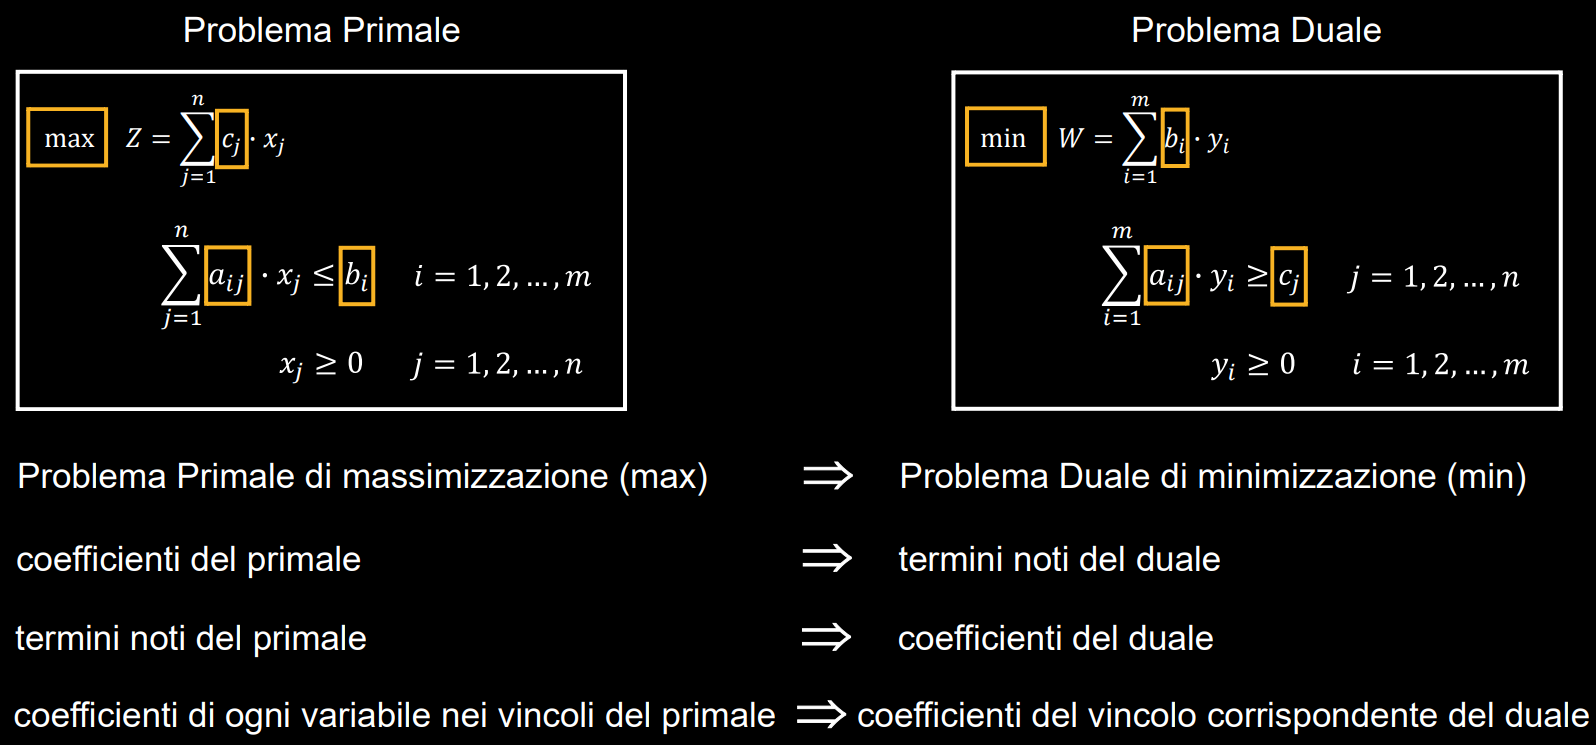
\includegraphics[width = 0.85\textwidth]{Images/44.png}
\end{center}
\subsubsection{Terminologia: caso base concreto, astratto e aggiunto}
Un \textbf{caso d'uso concreto} viene iniziato da un'attore ed esegue \textbf{l'intero comportamento desiderato dall'attore} [RUP]
Questi sono i \textbf{casi d'uso EBP}, che descrivono processi di business elementari.
Un caso \textbf{caso d'uso astratto} non viene \textbf{mai istanziato per se} ma si tratta invece di una \textbf{sottofunzione che fa parte di un'altro caso d'uso}.
Un caso d'uso che \textbf{include o è esteso da un'altro caso d'uso} è detto \textbf{caso d'uso base}; mentre il caso d'uso che è un estensione o inclusione è detto \textbf{caso d'uso aggiunto}.
I casi d'uso aggiunti sono \textbf{di solito astratti} mentre i casi d'uso base sono di solito \textbf{concreti}.
\subsubsection{Relazione di estensione}
Si supponga che il testo di un caso d'uso \textbf{non debba essere modificato} (almeno non in modo significativo) per qualche ragione.
Per esempio, perché modificare il caso d'uso con estensioni e modifiche risulta \textbf{difficile e poco manutenibile}.
Come possiamo aggiungere qualcosa al caso d'uso senza modificarlo?
La \textbf{relazione di estensione} offre una risposta a questa domanda. L'idea è quella di \textbf{creare un caso d'uso di estensione} (o aggiunto) e al suo interno descrivere \textbf{come modifica ed estende il comportamento del caso d'uso base}.
Un caso d'uso d'estensione è \textbf{attivato da una certa condizione trigger} e viene "eseguito" solo se \textbf{la condizione di estensione è vera}.
I punti di estensione sono \textbf{etichette nel caso d'uso base} a cui il caso d'uso d'estensione fa riferimento come \textbf{punto d'estensione}, cosicché la numerazione in passi del caso d'uso base può \textbf{cambiare senza influire sul caso d'uso d'estensione}.
L'extend può essere usata anche per la \textbf{gestione di eventi asincroni} e quando \textbf{il caso d'uso è chiuso rispetto a qualsiasi modifica}.
Il caso d'uso base \textbf{non dipende, per la sua esecuzione, dal caso d'uso aggiunto}; esso è un caso d'uso intero di per sé e per tanto \textbf{non definisce o controlla le condizioni in cui vengono attivate le estensioni}.
Alcune linee guida suggeriscono di usare la relazione extend e i casi d'uso di estensione \textbf{per modellare il comportamento condizionale o opzionale inserito nel caso d'uso base}, tuttavia ciò non coglie l'obbiettivo per il quale il comportamento opzionale e condizionale può \textbf{semplicemente essere registrato come testo nella sezione estensioni del caso d'uso base}.

\end{document}
